% (c) 2012 - 2014 - Dimitrios Vrettos d.vrettos@gmail.com
\chapter{Sistemi di equazioni}
\section{Equazione lineare in due incognite}

\begin{definizione}
Una equazione di primo grado (in $n$ incognite) si chiama \emph{equazione lineare}.
\end{definizione}

\begin{problema}
Determinare due numeri naturali la cui somma sia~16.
\end{problema}

\begin{soluzione}
L'ambiente del problema è l'insieme~$\insN$ dei numeri naturali. Indicati con~$x$ e~$y$ i due numeri
richiesti dal quesito, il problema si formalizza con l'equazione~$x+y=16$, equazione in due incognite, di
primo grado.

Determiniamo l'Insieme Soluzione del problema proposto.
L'obiettivo è trovare~$x\in\insN$ e~$y\in\insN$ tali che~$x+y=16$ oppure~$(x;y)\in\insN\times\insN\mid x+y=16$.
Le coppie di numeri naturali che sono soluzioni
dell'equazione sono facilmente determinabili e sono
tutte quelle riportate nella tabella seguente.

\begin{tabular}{cccccccccccccccccccc}
\toprule
$x$ & 0 & 1 & 2 & 3 & 4 & 5 & 6 & 7 & 8 & 9 & 10 & 11 & 12 & 13 & 14 & 15 & 16\\
$y$ & 16 & 15 & 14 & 13 & 12 & 11 & 10 & 9 & 8 & 7 & 6 & 5 & 4 & 3 & 2 & 1 & 0\\
\bottomrule
\end{tabular}\vspace{1.10ex}

L'Insieme Soluzione del problema posto è dunque
formato dalle~17 coppie di numeri naturali sopra elencate.
Riformuliamo il problema cercando coppie di numeri razionali la cui
somma sia~16.
In simboli scriviamo~$x\in\insQ$ e~$y\in\insQ$ tali che~$x+y=16$ oppure~$(x;y)\in\insQ\times\insQ\mid  x+y=16$.

Possiamo subito dire che tutte le coppie precedenti sono soluzione del
problema, ma ce ne sono infinite altre, ad esempio la coppia~$(-7;+23)$ è soluzione del problema perché sostituendo a~$x$ il
valore~$-7$ e a~$y$ il valore~$+23$ si ha~$(-7)+(+23)=16$.
Dal procedimento si capisce che anche la coppia~$(+23;-7)$ è
soluzione del problema perché~$(+23)+(-7)=16$.

Se attribuiamo un valore arbitrario a~$x$, l'altro
elemento della coppia soluzione si può ottenere sottraendo da~16 il
valore di~$x$:~~$y=16-x$.

Completa tu:

\begin{itemize*}
\item se~$x=-3$ allora~$y=16-(-3)=\ldots\ldots$ e la coppia (\ldots; \ldots) è soluzione dell'equazione;
\item se~$x=\frac{3}{2}$ allora~$y =\dotfill$, la coppia (\ldots\ldots; \ldots\ldots) è soluzione dell'equazione;
\item se~$x =\dotfill$ allora~$y=$ \dotfill, la coppia (\ldots\ldots; \ldots\ldots) è soluzione dell'equazione;
\item se~$x=\dotfill$allora~$y =$ \dotfill, la coppia (\ldots\ldots; \ldots\ldots) è soluzione dell'equazione.
\end{itemize*}

Quindi, se l'ambiente del problema è
l'insieme~$\insQ$, troviamo infinite coppie di
numeri razionali che soddisfano il problema.
E ancora, se formuliamo il problema nell'insieme dei
numeri reali~$\insR$, troveremo tutte le infinite coppie
soluzione del problema: basta assegnare all'incognita~$x$
valori reali arbitrari e determinare di conseguenza il corrispondente
valore di~$y=16-x$.

Se~$x=\sqrt{2}\Rightarrow y=16-\sqrt{2}$, quindi la coppia~$\left(\sqrt{2};16-\sqrt{2}\right)$ è soluzione
dell'equazione. 
\pagebreak

Completa:

\begin{itemize*}
\item se~$x=-2\sqrt{3}+1$ allora~$y=\dotfill$
\item se~$x=16+\frac{3\sqrt{5}}{2}$ allora~$y=\dotfill$
\end{itemize*}
\end{soluzione}

\begin{definizione}
Si chiama \emph{Insieme Soluzione} $(\IS)$ di un'equazione di primo
grado in due incognite $x$ e $y$, l'\emph{insieme delle coppie
ordinate} di valori che sostituiti rispettivamente a~$x$ e
a~$y$ rendono vera l'uguaglianza.
\end{definizione}

\ovalbox{\risolvii \ref{ese:19.1}, \ref{ese:19.2}, \ref{ese:19.3}}

\subsection{Rappresentazione di un'equazione lineare sul piano cartesiano}

\begin{exrig}\vspace{1.10ex}
 \begin{esempio}
Determinare l'insieme soluzione dell'equazione~$3y-x+1=0$ con~$x\in\insR$ e~$y\in\insR$.
 \end{esempio}
Osserviamo che l'equazione assegnata ha due incognite ed
è di primo grado; l'insieme soluzione sarà formato
dalle infinite coppie ordinate~$(x;y)$ di numeri tali che~$3y-x+1=0$.

Possiamo verificare che la coppia~$(1;0)$ è soluzione
dell'equazione, ma come facciamo a determinare tutte le
coppie che soddisfano quella equazione?

Fissiamo l'attenzione sull'incognita~$y$,
pensiamo l'equazione come un'equazione
nella sola~$y$, ricaviamo~$y$ come abbiamo fatto nelle equazioni di primo
grado ad una sola incognita, applicando i principi di equivalenza delle
equazioni:

\begin{equation*}
3y-x+1=0\:\Rightarrow\: 3y=x-1\:\Rightarrow\:\frac{3y}{3}=\frac{x-1}{3}\:\Rightarrow\: y=\frac{1}{3}x-\frac{1}{3}.
\end{equation*}

Dunque, al variare di~$x$ in~$\insR$, si ottengono tutte le infinite
soluzioni dell'equazione assegnata.
Prova a determinarne alcune:
\begin{center}
 \begin{tabular}{ccc}
\toprule
$x$ & $y$ & coppia\\
\midrule
$0$ &\ldots\ldots & ($0$;\ldots\ldots)\\
1& \ldots\ldots &($1$;\ldots\ldots)\\
$-1$ & \ldots\ldots & ($-1$;\ldots\ldots)\\
\bottomrule
\end{tabular}
\end{center}

In verità non possiamo elencare tutte le infinite coppie che risolvono
quella equazione, ma possiamo darne una rappresentazione grafica.

\begin{wrapfigure}{o}{0pt}
 % (c) 2012 Dimitrios Vrettos - d.vrettos@gmail.com
\begin{tikzpicture}[font=\small,x=5mm, y=5mm]

\draw[help lines,orange, dotted] (-3,-3) grid [step=1](5,5);

\begin{scope}[thick,->]
\draw (0,-3) -- (0,5) node[below left] {$y$};
\draw (-3,0) -- (5,0) node[below left] {$x$};
\end{scope}

\end{tikzpicture}




\end{wrapfigure}

La formula \[y=\frac{1}{3}x-\frac{1}{3}\] rappresenta una funzione
lineare; riportiamo le coppie trovate in un riferimento cartesiano
ortogonale e tracciamo la retta che rappresenta la funzione.

Una qualunque equazione lineare~$ax+by+c=0$ ammette infinite
soluzioni, costituite da coppie ordinate di numeri reali; esse sono le
coordinate cartesiane dei punti della retta grafico della funzione~$y=-{\dfrac{a}{b}}x-\dfrac{c}{b}$.
La formula~~$y=-{\dfrac{a}{b}}x-\dfrac{c}{b}$~~si chiama \emph{equazione esplicita della retta}.

\begin{esempio}
 Risolvi graficamente l'equazione~$y+\dfrac{2}{3}x-2=0\text{, con }x\in\insR\text{ e }y\in\insR$.
\end{esempio}

\begin{wrapfloat}{figure}{r}{0pt}
% (c) 2012 Dimitrios Vrettos - d.vrettos@gmail.com
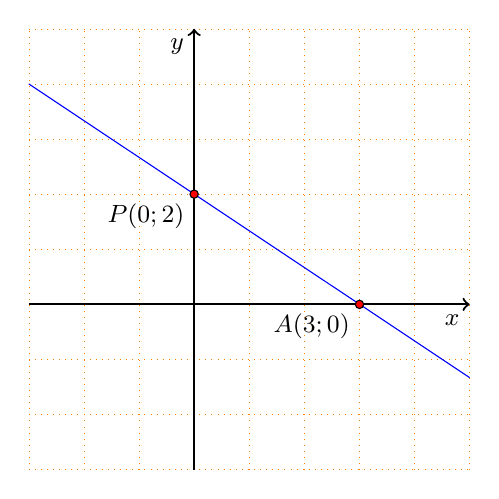
\begin{tikzpicture}[font=\small,x=7mm, y=7mm]

\draw[help lines,orange, dotted] (-3,-3) grid [step=1](5,5);

\begin{scope}[thick,->]
\draw (0,-3) -- (0,5) node[below left] {$y$};
\draw (-3,0) -- (5,0) node[below left] {$x$};
\end{scope}

\draw[blue] (-3,4) -- (5,-1.33);

\draw[fill=red] (0,2) circle (1.5pt) node[below left] {$P(0;2)$};
\draw[fill=red] (3,0) circle (1.5pt) node[below left] {$A(3;0)$};
\end{tikzpicture}

\end{wrapfloat}

L'equazione assegnata è in due incognite, di primo
grado, è cioè una equazione lineare. Nel riferimento cartesiano
ortogonale essa rappresenta una retta.

Troviamo l'equazione esplicita della retta:
\[y+\frac{2}{3}x-2=0\:\Rightarrow\: y=-{\frac{2}{3}}x+2.\]

Individuiamo l'ordinata del punto di intersezione della
retta con l'asse~$y$:~$q=2$, quindi~$P(0;2)$ è un
punto della retta.

Troviamo un altro punto appartenente alla retta: se~$x=3$ allora~$y=0$,
quindi~$A(3;0)$ è un punto della retta.

Disegniamo la retta nel piano cartesiano: le coppie~$(x;y)$, coordinate
dei punti della retta tracciata, sono le infinite soluzioni
dell'equazione assegnata.
\vspace{1.10ex}\end{exrig}

\ovalbox{\risolvii \ref{ese:19.4}, \ref{ese:19.5}, \ref{ese:19.6}}

\section{Risoluzione di sistemi di equazioni lineari}
\begin{problema}
\label{pr:19.1}
Nel rettangolo~$ABCD$, la somma del doppio di~$\overline{AB}$ con la metà di~$\overline{BC}$ è
di~$98\unit{m}$; aumentando~$\overline{AB}$ di~$3\unit{m}$ e~$\overline{BC}$ di~$2\unit{m}$, il perimetro del rettangolo
diventa di~$180\unit{m}$. Determinare l'area in~$\unit{m}^{2}$ del rettangolo.
\end{problema}
\begin{multicols}{2}
\emph{Dati}:
\begin{align*}
&2\overline{AB}+\frac{1}{2}\overline{BC}=98\unit{m}\text{,}\\
&2(\overline{AB}+3+\overline{BC}+2)=180\unit{m}.
\end{align*}

\emph{Obiettivo}: Area

\begin{center}
 % (c) 2012 Dimitrios Vrettos - d.vrettos@gmail.com
\begin{tikzpicture}[font=\small,x=2mm, y=2mm]
	\draw (0,0) rectangle  (9.6,7.4);

\node [below left] at (0,0) {$A$};
\node[above left]  at (0,7.4) {$B$};
\node[below right]  at (9.6,0) {$D$};
\node[above right]  at (9.6,7.4) {$C$};
\end{tikzpicture}
\end{center}
\end{multicols}
 \begin{soluzione}
Per determinare l'area del rettangolo dobbiamo
moltiplicare le misure delle sue dimensioni~$\Area=\overline{AB}\cdot\overline{BC}$
che però non conosciamo; il problema ha quindi due incognite.

Analizzando i dati possiamo osservare che ci sono fornite due
informazioni che legano le grandezze incognite. Se poniamo~$\overline{AB}=x$ e~$\overline{BC}=y$
otteniamo le due equazioni:
\[2x+\frac{1}{2}y=98;\quad~2(x+3+y+2)=180\]
che dovranno risultare soddisfatte per una stessa coppia di numeri
reali.
 \end{soluzione}

 \begin{definizione}
Si definisce \emph{sistema di equazioni} l'insieme di più equazioni, in due o più incognite,
che devono essere verificate contemporaneamente. La scrittura formale
si ottiene raggruppando le equazioni mediante una parentesi graffa.
\end{definizione}

Analizzeremo in particolare i sistemi in due equazioni e due incognite.

\begin{definizione}
L'Insieme Soluzione ($\IS$) di un sistema di equazioni in
due incognite è formato da tutte le coppie di valori
che rendono contemporaneamente vere tutte le equazioni del sistema.
\end{definizione}

\begin{definizione}
Si chiama \emph{grado di un sistema} il prodotto dei gradi delle
equazioni che lo compongono. In particolare, se le equazioni che lo
compongono sono di primo grado, il sistema si chiama \emph{sistema lineare}.

La \emph{forma normale} o \emph{canonica} di un sistema lineare è:
\[\left\{\begin{array}{l}a_{1}x+b_{1}y=c_{1}\\
a_{2}x+b_{2}y=c_{2} \end{array}\right.\text{, con }a_{1}\text{,~}b_{1}\text{,~}c_{1}\text{,~}a_{2}\text{,~}b_{2}\text{ e }c_{21}\text{ numeri reali.}\]
\end{definizione}

Il problema \ref{pr:19.1} si formalizza dunque con il sistema
\[\longarray\left\{\begin{array}{l}2x+\dfrac{1}{2}y=98
\\2(x+3+y+2)=180\end{array}\right.\]
composto da due equazioni in due incognite di primo grado e pertanto il suo grado
è~1 (è un sistema lineare). La sua forma canonica si ottiene
sviluppando i calcoli nella seconda equazione
\[\longarray\left\{\begin{array}{l}2x+\dfrac{1}{2}y=98\\
2x+2y=170 \end{array}\right..\]

\subsection{Procedimento per ottenere la forma canonica di un sistema}
La forma canonica di un sistema lineare di due equazioni in due
incognite è, come abbiamo visto,
\[\left\{\begin{array}{l}a_{1}x+b_{1}y=c_{1}
\\a_{2}x+b_{2}y=c_{2} \end{array}\right.\]
con~$a_{1}$, $b_{1}$, $c_{1}$, $a_{2}$, $b_{2}$ e $c_{2}$ numeri reali.

\begin{exrig}
 \begin{esempio}
 Scrivere in forma canonica il sistema:
\[\longarray\left\{\begin{array}{l}4x^{2}-(y+2x)^{2}=x+1-y(4x+y-1)\\
\dfrac{x-2}{2}+\dfrac{y+3}{3}=0
\end{array}\right..\]

Eseguiamo i calcoli nella prima equazione e riduciamo allo stesso
denominatore la seconda equazione:

\[\left\{\begin{array}{l}
 4x^{2}-y^{2}-4x^{2}-4xy=x+1-4xy-y^{2}+y\\
 3x-6+2y+6=0
 \end{array}\right..\]

Per mezzo del primo principio di equivalenza delle equazioni portiamo le
incognite al primo membro e sommiamo i termini simili, ottenendo
 \[\left\{\begin{array}{l}
   x+y=-1\\
   3x+2y=0
\end{array}\right.\]
che è la forma canonica cercata.
 \end{esempio}
\end{exrig}

\subsection{Metodo di sostituzione}
\emph{Risolvere il sistema} significa determinare tutte le coppie di
numeri reali che soddisfano contemporaneamente le due equazioni.

Analizziamo i diversi metodi che permettono di ottenere
l'Insieme Soluzione, cominciamo dal \emph{metodo di sostituzione}.

\begin{exrig}
\begin{esempio}
$\left\{\begin{array}{l}-3x+y=2\\5x-2y=7\end{array}\right.$.
\end{esempio}

Il sistema si presenta già in forma canonica. Il metodo di
sostituzione si svolge nei seguenti passi:

\paragraph{Passo I} scegliamo una delle due equazioni e una
delle due incognite da cui partire. Applicando i principi
d'equivalenza delle equazioni, ricaviamo questa
incognita.
Nel nostro esempio, partiamo dalla prima equazione e ricaviamo
l'incognita~$y$
\[\left\{\begin{array}{l}
     -3x+y=2\\
     5x-2y=7
    \end{array}
\right.
\Rightarrow
\left\{\begin{array}{l}y=2+3x \\
	 5x-2y=7
\end{array}\right..\]

\paragraph{Passo II} sostituiamo nella seconda equazione, al posto
dell'incognita trovata, l'espressione
a cui essa risulta uguale dalla prima equazione. Nel nostro esempio abbiamo
\[\left\{\begin{array}{l}
     y=2+3x\\
     5x-2y=7
    \end{array}
\right.
\Rightarrow
\left\{\begin{array}{l}y=2+3x \\
	 5x-2(2+3x)=7
\end{array}\right..\]

\paragraph{Passo III} svolgiamo i calcoli nella seconda equazione.
Nel nostro esempio
\[\left\{\begin{array}{l}y=2+3x\\
5x-4-6x=7\end{array}\right..\]

\paragraph{Passo IV} risolviamo la seconda equazione, che ora è
un'equazione di primo grado in una sola variabile.
Nel nostro esempio, ricaviamo~$x$ dalla seconda equazione
\[\left\{\begin{array}{l}
	 y=2+3x\\
	 5x-4-6x=7
	\end{array}\right.\Rightarrow
 \left\{\begin{array}{l}y=2+3x\\
	 -x=7+4
	\end{array}\right.\Rightarrow
 \left\{\begin{array}{l}y=2+3x\\
	 x=-11
  \end{array}\right..\]

\paragraph{Passo V} sostituiamo nella prima equazione il valore
numerico dell'incognita trovata e avremo
un'equazione di primo grado nell'altra incognita. Risolviamo
quest'ultima equazione.
Nel nostro esempio
\[ \left\{\begin{array}{l}y=2+3x\\
	 x=-11
  \end{array}\right.\Rightarrow
  \left\{\begin{array}{l}
	 y=-31\\
	 x=-11
  \end{array}\right..\]

\paragraph{Passo VI} possiamo ora scrivere l'insieme soluzione.
Nel nostro esempio~$\IS=\{(-11;-31)\}$.

In conclusione, il sistema è \emph{determinato}, la coppia ordinata
$(-11;-31)$ verifica contemporaneamente le due equazioni del sistema.

\begin{esempio}
$\longarray\left\{\begin{array}{l}
	\dfrac{1}{2}(x-1)+3\left(y+\dfrac{1}{3}\right)=\dfrac{1}{6}\\
	y\left(1+\dfrac{2}{5}\right)-2=\dfrac{4}{5}-\dfrac{x-1}{5}
	\end{array}\right..$

\begin{enumeratea}
 \item Il sistema non si presenta nella forma canonica. Svolgiamo i calcoli e portiamo il sistema in forma canonica:
\[\longarray\left\{\begin{array}{l}3x+18y=-2\\x+7y=15\end{array}\right.;\]
\item ricaviamo~$x$ dalla seconda equazione:
\[\longarray\left\{\begin{array}{l}3x+18y=-2\\x=15-7y\end{array}\right.;\]
\item abbiamo fatto questa scelta perché possiamo ottenere il valore di~$x$
con facilità e senza frazioni. Sostituiamo nella prima equazione al posto di~$x$
l'espressione trovata:
\[\longarray\left\{\begin{array}{l}
          3\cdot(15-7y)+18y=-2\\
          x=15-7y
          \end{array}\right.;
\]
\item risolviamo la prima equazione che è di primo grado nella sola
incognita~$y$:
\[\left\{\begin{array}{l}
          -3y=-47\\
          x=15-7y
          \end{array}\right.
\Rightarrow\longarray\left\{\begin{array}{l}
          y=\dfrac{47}{3}\\
          x=15-7y
         \end{array}\right.;\]
\item sostituiamo il valore di~$y$ nella seconda equazione:
\[\longarray\left\{\begin{array}{l}
          y=\dfrac{47}{3}\\
          x=15-7\left(\dfrac{47}{3}\right)
          \end{array}\right.
\Rightarrow \longarray\left\{\begin{array}{l}x=-\dfrac{284}{3}\\
 y=\dfrac{47}{3}\end{array}\right..\]
\end{enumeratea}

Possiamo scrivere l'insieme delle soluzioni:
\[\IS=\left\{\left(-\frac{284}{3};\frac{47}{3}\right)\right\}.\]

In conclusione, il sistema è \emph{determinato}; la coppia
ordinata~$\left(-\frac{284}{3};\frac{47}{3}\right)$ verifica contemporaneamente le due
equazioni del sistema.
 \end{esempio}

 \begin{esempio}
 $\longarray\left\{\begin{array}{l}
 \dfrac{1}{y}=2\left(\dfrac{x}{y}-\dfrac{1}{2}\right)\\
 \dfrac{5x+4y+19}{x}=-2\end{array}\right..$

 Il sistema è fratto poiché in ciascuna equazione compare
l'incognita al denominatore; per poter applicare il
secondo principio di equivalenza delle equazioni eliminando i
denominatori, dobbiamo porre le~$\CE$ e individuare il Dominio $\Dom$ del sistema
assegnato, cioè l'insieme in cui si troverà~$\CE: y\neq~0\text{ e }x\neq~0$ per
cui~$\Dom=\insR_{0}\times \insR_{0}$.

Portiamo a forma canonica applicando i principi di equivalenza delle
equazioni:

\begin{equation*}
{\longarray\left\{\begin{array}{l}
	  \dfrac{1}{y}=2\left(\dfrac{x}{y}-\dfrac{1}{2}\right)\\
	  \dfrac{5x+4y+19}{x}=-2\end{array}\right.\Rightarrow
 \left\{\begin{array}{l}
	  \dfrac{1}{y}=\dfrac{2x}{y}-1\\
	  5x+4y+19=-2x\end{array}\right.}\Rightarrow
 \left\{\begin{array}{l}
	  2x-y=1\\
	  7x+4y=-19\end{array}\right..
\end{equation*}

Applichiamo il metodo di sostituzione:

\begin{multline*}
\left\{\begin{array}{l}2x-y=1\\7x+4y=-19\end{array}\right.\Rightarrow
\left\{\begin{array}{l}y=2x-1\\7x+4y=-19\end{array}\right.\Rightarrow
\left\{\begin{array}{l}y=2x-1\\7x+4(2x-1)=-19\end{array}\right.
\\\Rightarrow
\left\{\begin{array}{l}y=2x-1\\15x=-15\end{array}\right.\Rightarrow
\left\{\begin{array}{l}y=2(-1)-1\\x=-1\end{array}\right.\Rightarrow
\left\{\begin{array}{l}y=-3\\x=-1\end{array}\right..
\end{multline*}
La soluzione $(-1;-3)$ è compatibile con le condizioni di esistenza.
\end{esempio}
 \end{exrig}

 \ovalbox{\risolvii \ref{ese:19.7}, \ref{ese:19.8}, \ref{ese:19.9}, \ref{ese:19.10}, \ref{ese:19.11}, \ref{ese:19.12}, \ref{ese:19.13}, \ref{ese:19.14}, \ref{ese:19.15}}

 \subsection{Metodo del confronto}

\begin{exrig}
\begin{esempio}
$\left\{\begin{array}{l}-3x+y=2\\5x-2y=7\end{array}\right..$

\paragraph{Passo I} ricaviamo da entrambe le equazioni la stessa
incognita. Nel nostro esempio ricaviamo la~$y$ contemporaneamente da entrambe le
equazioni:
\[\left\{\begin{array}{l}y=2+3x\\y=\dfrac{5x-7}{2}\end{array}\right..\]

\paragraph{Passo II} poiché il primo membro delle
equazioni è lo stesso, possiamo uguagliare anche i secondi membri,
ottenendo un'equazione in una incognita. Nell'esempio~$2+3x=\dfrac{5x-7}{2}.$

\paragraph{Passo III} risolviamo l'equazione trovata e determiniamo il valore di una delle due incognite.
Nel nostro esempio~$4+6x=5x-7\:\Rightarrow\: x=-11$.

\paragraph{Passo IV} si sostituisce il valore trovato
dell'incognita in una delle due equazioni e ricaviamo
l'altra incognita. Nel nostro esempio:
\[\left\{\begin{array}{l}
     x=-11\\
     y=2+3x
     \end{array}\right.
\Rightarrow\left\{\begin{array}{l}
          x=-11\\
          y=-31
         \end{array}\right..\]
\paragraph{Passo V} possiamo ora scrivere l'insieme soluzione.
Nel nostro esempio:~$\IS=\{(-11;-31)\}$.

In conclusione, il sistema è determinato, la coppia ordinata~$(-11;-31)$
verifica contemporaneamente le due equazioni del sistema.
 \end{esempio}
\end{exrig}

\ovalbox{\risolvii \ref{ese:19.16}, \ref{ese:19.17}, \ref{ese:19.18}, \ref{ese:19.19}}

\subsection{Metodo di riduzione}
Il metodo di riduzione si basa sulla seguente osservazione: se un
sistema è formato dalle equazioni~$A=B$ e~$C=D$, possiamo dedurre
da queste la nuova equazione~$A+C=B+D$ ad esse equivalente.
\begin{equation*}
\left\{\begin{array}{l}A=B \\C=D
\end{array}\right.\:\Rightarrow\: A+C=B+D.
\end{equation*}
L'equazione ottenuta potrebbe presentarsi in una sola
incognita e quindi potrebbe essere facile trovare il valore di quella
incognita.

\begin{exrig}
 \begin{esempio}
$\left\{\begin{array}{l}3x-5y=1 \\2x+5y=-4\end{array}\right..$

Sommando membro a membro le due equazioni otteniamo~$(3x-5y)+(2x+5y)=1-4$.
I termini in~$y$ si eliminano perché opposti. Sommando i monomi simili
si ha~$5x=-3\Rightarrow x=-{\frac{3}{5}}$.
 \end{esempio}
\end{exrig}

Questo metodo, applicato semplicemente sommando membro a membro le
equazioni, funziona solo se i coefficienti di una delle due incognite
sono opposti. Solo in questo caso sommando le equazioni una delle due
incognite ``sparisce''. Tuttavia con
qualche accorgimento è possibile applicarlo in ogni caso.

Sfruttiamo il secondo principio di equivalenza delle equazioni che ci
permette di moltiplicare ambo i membri di un'equazione
per uno stesso numero diverso da zero. In questo modo possiamo sempre
trasformare le due equazioni affinché l'incognita~$x$
appaia con coefficienti opposti nella prima e nella seconda equazione.


\begin{exrig}
 \begin{esempio}
$\left\{\begin{array}{l}3x-5y=1\\5x-4y=-4\end{array}\right..$

Nel nostro esempio possiamo moltiplicare la prima equazione per~5 e la
seconda per~$-3$, ottenendo:
 \[\begin{array}{l}+5\\-3\end{array}
 \left\{\begin{array}{l}3x-5y=1\\5x-4y=-4\end{array}\right.\Rightarrow
 \left\{\begin{array}{l}15x-25y=5\\-15x+12y=12\end{array}\right.;\]
sommando membro a membro abbiamo
\begin{equation*}
(15x-25y)+(-15x+12y)=5+12\quad\Rightarrow\quad -13y=17\quad\Rightarrow\quad
y=-{\frac{17}{13}}.
\end{equation*}

Dopo aver determinato il valore di una incognita possiamo sostituirlo in
una qualsiasi equazione del sistema e determinare il valore
dell'altra incognita o ripetere il procedimento per l'altra incognita moltiplicando come segue:
\[\begin{array}{l}+4\\-5\end{array}\left\{\begin{array}{l}3x-5y=1\\5x-4y=-4\end{array}\right.
\Rightarrow\left\{\begin{array}{l}12x-20y=4\\-25x+20y=20\end{array}\right..\]
Sommando le due equazioni otteniamo~$-13x=24\:\Rightarrow\: x=-{\dfrac{24}{13}}$.

Abbiamo così determinato la coppia soluzione del sistema~$\left(-{\dfrac{24}{13}};-\dfrac{17}{13}\right)$.
 \end{esempio}
\end{exrig}

\subsubsection{Generalizzazione del metodo di riduzione}

Assegnato il sistema lineare~$\left\{\begin{array}{l}a_{1}x+b_{1}y=c_{1}\\a_{2}x+b_{2}y=c_{2} \end{array}\right.$
con~$a_{1}$, $b_{1}$, $c_{1}$, $a_{2}$, $b_{2}$, $c_{2}$ numeri reali.

\paragraph{Passo I} per eliminare~$y$ moltiplichiamo la prima equazione per~$b_{2}$ e la seconda per~$-b_{1}$:
\[\left\{\begin{array}{l}a_{1}b_{2}x+b_{1}b_{2}y=c_{1}b_{2}\\-a_{2}b_{1}x-b_{1}b_{2}y=-b_{1}c_{2}\end{array}\right..\]

\paragraph{Passo II} sommiamo le due equazioni:
\[a_{1}b_{2}x-a_{2}b_{1}x=c_{1}b_{2}-b_{1}c_{2}\quad\Rightarrow\quad (a_{1}b_{2}-a_{2}b_{1})x=c_{1}b_{2}-b_{1}c_{2}.\]

\paragraph{Passo III} ricaviamo l'incognita~$x$:
 \[x=\frac{c_{1}b_{2}-b_{1}c_{2}}{a_{1}b_{2}-a_{2}b_{1}}\text{,~~con }a_{1}b_{2}-a_{2}b_{1}\neq~0.\]

\paragraph{Passo IV} per eliminare~$x$ moltiplichiamo la prima equazione per~$-a_{2}$ e la seconda per~$a_{1}$:
\[\left\{\begin{array}{l}-a_{1}a_{2}x-a_{2}b_{1}y=-a_{2}c_{1}\\a_{1}a_{2}x+a_{1}b_{2}y=a_{1}c_{2}\end{array}\right.\]

\paragraph{Passo V} sommiamo le due equazioni
\[-a_{2}b_{1}y+a_{1}b_{2}y=-a_{2}c_{1}+a_{1}c_{2}\quad\Rightarrow\quad
(a_{1}b_{2}-a_{2}b_{1})y=a_{1}c_{2}-a_{2}c_{1}.\]

\paragraph{Passo VI} ricaviamo l'incognita~$y$:
\[y=\frac{a_{1}c_{2}-a_{2}c_{1}}{a_{1}b_{2}-a_{2}b_{1}}\text{,~~con }a_{1}b_{2}-a_{2}b_{1}\neq~0.\]

La soluzione è
\[\left(\frac{c_{1}b_{2}-b_{1}c_{2}}{a_{1}b_{2}-a_{2}b_{1}};\frac{a_{1}c_{2}-a_{2}c_{1}}{a_{1}b_{2}-a_{2}b_{1}}\right)\text{,~~con }a_{1}b_{2}-a_{2}b_{1}\neq~0.\]

\ovalbox{\risolvii \ref{ese:19.20}, \ref{ese:19.21}, \ref{ese:19.22}, \ref{ese:19.23}}

\subsection{Metodo di Cramer}

\begin{definizione}
Si chiama \emph{matrice del sistema lineare} di due equazioni in due incognite la tabella
\[\left[\begin{array}{cc}a_{1} & b_{1}\\a_{2} & b_{2}\end{array}\right]\]
in cui sono sistemati i coefficienti delle incognite del sistema
posto in forma canonica; si~chiama \emph{determinante della matrice} il numero reale
\[D=\left|\begin{array}{cc}a_{1} & b_{1} \\ a_{2} & b_{2}\end{array}\right|=a_{1}\cdot b_{2}-b_{1}\cdot a_{2}\]
ad essa associato.
\end{definizione}

Dalla generalizzazione del metodo di riduzione, abbiamo visto che la soluzione del sistema è data da

\begin{equation*}
\left(\dfrac{c_{1}b_{2}-b_{1}c_{2}}{a_{1}b_{2}-a_{2}b_{1}};\dfrac{a_{1}c_{2}-a_{2}c_{1}}{a_{1}b_{2}-a_{2}b_{1}}\right)\text{,~~con }a_{1}b_{2}-a_{2}b_{1}\neq~0
\end{equation*}
ovvero
\begin{equation*}
\left(\dfrac{c_{1}b_{2}-b_{1}c_{2}}{D};\dfrac{a_{1}c_{2}-a_{2}c_{1}}{D}\right)\text{,~~con }D\neq~0
\end{equation*}
quindi possiamo dedurre che:
un \emph{sistema lineare} è \emph{determinato}, ammette cioè una
sola coppia soluzione, \emph{se il determinante della matrice del sistema è diverso da zero}.

\vspazio\ovalbox{\risolvii \ref{ese:19.24}, \ref{ese:19.25}}\vspazio

La \emph{regola di Cramer}\footnote{dal nome del matematico svizzero Gabriel Cramer
(1704 - 1752).} (o \emph{metodo do Cramer}) ci permette di stabilire la coppia soluzione di un sistema
lineare di due equazioni in due incognite, costruendo e calcolando tre
determinanti:

\begin{enumeratea}
\item $D$ il determinante della matrice del sistema:
 \[D=\left|\begin{array}{cc}a_{1} & b_{1}\\ a_{2} & b_{2}\end{array}\right|=a_{1}\cdot b_{2}-b_{1}\cdot a_{2};\]
\item $D_{x}$ il determinante della matrice ottenuta sostituendo agli
elementi della prima colonna di $D$ i termini noti.
\[D_{x}=\left|\begin{array}{cc}c_{1} & b_{1}\\ c_{2} & b_{2}\end{array}\right|=c_{1}\cdot b_{2}-b_{1}\cdot c_{2};\]
\item $D_{y}$ il determinante della matrice ottenuta sostituendo agli
elementi della seconda colonna di $D$ i termini noti. 
\[D_{y}=\left|\begin{array}{cc}a_{1} & c_{1}\\ a_{2} & c_{2}\end{array}\right|=a_{1}\cdot c_{2}-c_{1}\cdot a_{2}.\] 
\end{enumeratea}

Se~$D\neq~0$ il sistema è determinato e la coppia
soluzione è
\begin{equation*}
\left(\frac{D_{x}}{D};\, \frac{D_{y}}{D}\right).
\end{equation*}

%\newpage
\begin{exrig}
 \begin{esempio}
$\left\{\begin{array}{l}2x+3y=4 \\4x-3y=2\end{array}\right.$.

Calcoliamo i determinanti $D$, $D_x$ e $D_y$.

 \[D=\left|\begin{array}{cc}a_{1} & b_{1}\\a_{2} & b_{2}\end{array}\right|=a_{1}\cdot b_{2}-b_{1}\cdot a_{2}\:\Rightarrow\:
 D=\left|\begin{array}{cc} 2 & 3 \\ 4 & -3\end{array}\right|=2\cdot (-3)-3\cdot 4=-6-12=-18.\]

Poiché $D\neq~0$ il sistema è determinato.

 \[D_{x}=\left|\begin{array}{cc}c_{1}& b_{1}\\c_{2} & b_{2}\end{array}\right|=c_{1}\cdot b_{2}-b_{1}\cdot c_{2}\:\Rightarrow\:
 D_{x}=\left|\begin{array}{cc}4 & 3\\2 & -3\end{array}\right|=4\cdot (-3)-3\cdot 2=-12-6=-18\text{,}\]

 \[D_{y}=\left|\begin{array}{cc}a_{1}& c_{1}\\a_{2} & c_{2}\end{array}\right|=a_{1}\cdot c_{2}-c_{1}\cdot a_{2}\:\Rightarrow\:
 D_{y}=\left|\begin{array}{cc}2 & 4\\4 & 2\end{array}\right|=2\cdot 2-4\cdot 4=4-16=-12.\]

\begin{equation*}
 x=\frac{D_{x}}{D}=\frac{-18}{-18}=1;\quad
 y=\frac{D_{y}}{D}=\frac{-12}{-18}=\frac{2}{3}.
 \end{equation*}
 \end{esempio}
\end{exrig}

\ovalbox{\risolvii \ref{ese:19.26}, \ref{ese:19.27}, \ref{ese:19.28}, \ref{ese:19.29}, \ref{ese:19.30}, \ref{ese:19.31}, \ref{ese:19.32}}

\subsection{Classificazione dei sistemi rispetto alle soluzioni}
Dato un sistema in forma canonica
$\left\{\begin{array}{l}a_{1}x+b_{1}y=c_{1}\\a_{2}x+b_{2}y=c_{2} \end{array}\right. $ ricordando
che:
\begin{align*}
& D=\left|\begin{array}{cc}a_{1} & b_{1}\\ a_{2} & b_{2}\end{array}\right|=a_{1}\cdot b_{2}-b_{1}\cdot a_{2};\\
& D_{x}=\left|\begin{array}{cc}c_{1} & b_{1}\\ c_{2} & b_{2}\end{array}\right|=c_{1}\cdot b_{2}-b_{1}\cdot c_{2};\\
& D_{y}=\left|\begin{array}{cc}a_{1} & c_{1}\\ a_{2} & c_{2}\end{array}\right|=a_{1}\cdot c_{2}-c_{1}\cdot a_{2};
\end{align*}


\begin{itemize*}
\item se $D \neq 0$ il sistema è \emph{determinato}: esiste una sola coppia soluzione~$x=\frac{D_{x}}{D}\text{, }y=\frac{D_{y}}{D}$;
\item se~$D=0$ si possono verificare due casi:
 \begin{itemize*}
\item 1$\grado$ caso: se~$D_{x}=0$ e~$D_{y}=0$ il sistema è \emph{indeterminato}: ogni
coppia di numeri reali che verifica un'equazione, verifica anche l'altra;
\item 2$\grado$ caso: se~$D_{x}\neq~0$ e~$D_{y} \neq~0$ il sistema è \emph{impossibile}: non
esiste alcuna coppia di valori che soddisfa entrambe le equazioni, cioè~$\IS=\emptyset $.
 \end{itemize*}
\end{itemize*}

\begin{exrig}
 \begin{esempio}
$\left\{\begin{array}{l}2x-3y=1 \\4x-3y=2 \end{array}\right..$

\[D=\left|\begin{array}{cc}2&-3\\4&-3\end{array}\right|=2\cdot (-3)+3\cdot (4)=-6+12=6\neq~0;\]
il sistema è determinato.
 \end{esempio}

 \begin{esempio}
$\left\{\begin{array}{l}8x-6y=2 \\4x-3y=1 \end{array}\right..$

\[D=\left|\begin{array}{cc}{8}&{-6}\\{4}&{-3}\end{array}\right|=8\cdot (-3)+6\cdot (4)=-24+24=0;\]
il sistema è indeterminato o impossibile.

\begin{align*}
& D_{x}=\left|\begin{array}{cc}{2}&{-6}\\{1}&{-3}\end{array}\right|=2\cdot(-3)-(-6)\cdot 1=-6+6=0;\\
& D_{y}=\left|\begin{array}{cc}{8}&{2}\\{4}&{1}\end{array}\right|=8\cdot1-2\cdot 4=8-8=0.
\end{align*}
Il sistema è indeterminato.
 \end{esempio}

 \begin{esempio}
$\left\{\begin{array}{l}8x-6y=1 \\4x-3y=2\end{array}\right..$


\[D=\left|\begin{array}{cc}{8}&{-6}\\{4}&{-3}\end{array}\right|=8\cdot(-3)-4\cdot (-6)=-24+24=0;\]
il sistema è indeterminato o impossibile.

\begin{align*}
& D_{x}=\left|\begin{array}{cc}{1}&{-6}\\{2}&{-3}\end{array}\right|=1\cdot(-3)-(-6)\cdot 2=-3+12=9;\\
& D_{y}=\left|\begin{array}{cc}{8}&{1}\\{4}&{2}\end{array}\right|=8\cdot2-1\cdot 4=16-4=12.
\end{align*}
Il sistema è impossibile.
 \end{esempio}
\end{exrig}
Osserviamo che se~$D=0$ si ha
\[a_{1}\cdot b_{2}-b_{1}\cdot a_{2}=0\quad\Rightarrow\quad a_{1}\cdot b_{2}=b_{1}\cdot a_{2}\quad\Rightarrow\quad\frac{a_{1}}{a_{2}}=\frac{b_{1}}{b_{2}}.\]
Ciò significa che, se i coefficienti delle incognite della prima equazione sono proporzionali
ai coefficienti delle incognite della seconda equazione allora il
sistema è indeterminato o impossibile.

In particolare, se poi~$D_{x}=0$ si ha
\[c_{1}\cdot b_{2}-b_{1}\cdot c_{2}=0\quad\Rightarrow\quad c_{1}\cdot b_{2}=b_{1}\cdot c_{2}\quad\Rightarrow\quad \frac{c_{1}}{c_{2}}=\frac{b_{1}}{b_{2}}.\]
Quindi se anche i termini noti delle due equazioni sono nella stessa proporzione,
cioè se
\[\frac{a_{1}}{a_{2}}=\frac{b_{1}}{b_{2}}=\frac{c_{1}}{c_{2}}\] il
sistema è indeterminato.

Se invece~$D_{x} \neq 0$, cioè
\[\frac{c_{1}}{c_{2}}\neq\frac{b_{1}}{b_{2}}\] il sistema è impossibile.

\vspazio\ovalbox{\risolvii \ref{ese:19.33}, \ref{ese:19.34}, \ref{ese:19.35}, \ref{ese:19.36}, \ref{ese:19.37}, \ref{ese:19.38}, \ref{ese:19.39}, \ref{ese:19.40}}

\subsection{Il metodo grafico}

Il problema della ricerca dell'Insieme Soluzione di
un'equazione lineare ci ha condotto ad un proficuo
collegamento tra concetti algebrici e concetti geometrici; in
particolare abbiamo visto che:

\begin{center}
 \begin{tabularx}{.9\textwidth}{XX}
\toprule
 Concetto algebrico & Concetto geometrico\\
 \midrule
Coppia ordinata di numeri reali & Punto del piano dotato di riferimento cartesiano\\
Equazione lineare & Retta \\
Coppia soluzione dell'equazione& Punto della retta di equazione \\
$ax+by+c=0$ & $y=-{\frac{a}{b}}x-\frac{c}{b}$\\
\bottomrule
 \end{tabularx}

\end{center}
Vedremo ora come sia possibile sfruttare questi collegamenti per
risolvere un sistema lineare di due equazioni in due incognite.

\begin{problema}
Determina due numeri reali di cui si sa che la loro somma è~6 e il
doppio del primo aumentato della metà del secondo è ancora~6.
\end{problema}

 \begin{soluzione}
Indichiamo con~$x$ e~$y$ i due numeri incogniti; il problema si formalizza
con due equazioni:~$x+y=6$ e~$2x+\frac{1}{2}y=6$.

Dobbiamo individuare una coppia di numeri reali che sia soluzione
dell'una e dell'altra equazione.

\paragraph{Il punto di vista algebrico}
La coppia di numeri reali~$x$ e~$y$ che risolve il problema è quella che
risolve il sistema
\[\longarray\left\{\begin{array}{l}x+y=6\\2x+\dfrac{1}{2}y=6 \end{array}\right..\]
Applicando uno qualunque dei metodi algebrici esposti si ottiene~$x=2$ e~$y=4$.

\paragraph{Il punto di vista geometrico}

Il problema si può spostare in ambiente geometrico: la coppia
soluzione rappresenta un punto che appartiene sia alla retta
rappresentata dalla prima equazione, sia alla retta rappresentata dalla
seconda equazione. Quindi rappresenta il punto di intersezione delle due rette.

Si rappresenta il sistema di rette nel riferimento cartesiano ortogonale.
La retta~$a$ è quella di equazione~$x+y=6$, che passa per i
punti~$(6;0)$ e~$(0;6)$.

La retta~$b$ è quella di equazione~$2x+\frac{1}{2}y=6$, che
passa per i punti~$(3;0)$ e~$(0;12)$.

Il punto~$A(2;4)$ è il punto di intersezione delle due rette, le sue
coordinate formano la coppia soluzione del sistema e di conseguenza
sono i due numeri che stiamo cercando nel problema.

\begin{center}
 % (c) 2012 Dimitrios Vrettos - d.vrettos@gmail.com
% (c) 2012 Dimitrios Vrettos - d.vrettos@gmail.com
\begin{tikzpicture}[scale=.7, x=10mm, y=10mm]
    \draw[dotted,color=orange] (-3,-2) grid (8,7);
    \draw[->] (-3,0) -- (8,0) node[below left] {$x$};
    \draw[->] (0,-2) -- (0,7) node[below left] {$y$};
    
\foreach \x/\xtext in {-2/-2,-1/-1,1/1,2/2,3/3,4/4,5/5,6/6,7/7}
\node[below]  at (\x,0) {$\xtext$};
\foreach \y/\ytext in {-1/-1,1/1,2/2,3/3,4/4,5/5,6/6}
\node[left] at (0,\y) {$\ytext$};

\foreach \xi in {-2,-1,...,7}
\draw (\xi,3pt) -- (\xi,-3pt);
\foreach \yi in {-1,0,...,6}
\draw (3pt,\yi) -- (-3pt,\yi);

\node [below left] at (0,0) {0};
\draw[color=red,domain=-.5:7.2] plot[id=x] function{6-x} 
        node[right] {$a$};
    
\draw[color=blue,domain=1.3:3.4] plot[id=x] function{12-4*x} 
        node[right] {$b$};
  \draw[fill=green] (2,4) circle (1.5pt) node[above right] {$A(2;4)$};
\end{tikzpicture}

\end{center}
 \end{soluzione}

 \begin{exrig}
 \begin{esempio}
$\left\{\begin{array}{l}2x-3y=7 \\x+y+6=5(x-y)\end{array}\right..$

\paragraph{Il punto di vista algebrico}
Portiamo in forma canonica il sistema, ottenendo:

\begin{equation*}
\left\{\begin{array}{l}2x-3y=7 \\x+y+6=5(x-y)\end{array}\right.\Rightarrow
\left\{\begin{array}{l}2x-3y=7 \\x+y+6=5x-5y\end{array}\right.\Rightarrow
\left\{\begin{array}{l}2x-3y=7 \\-4x+6y=-6\end{array}\right..
\end{equation*}

Si può notare che il sistema ha i coefficienti delle incognite in
proporzione:
\[\frac{a_{1}}{a_{2}}=\frac{2}{-4}=-{\frac{1}{2}}\quad\text{e}\quad\frac{b_{1}}{b_{2}}=\frac{-3}{+6}=-{\frac{1}{2}}\text{,}\]
mentre i termini noti non sono nella stessa proporzione
\[\frac{c_{1}}{c_{2}}=\frac{7}{-1}\text{,}\]
quindi il sistema è impossibile:~$\IS=\emptyset $.

\paragraph{Il punto di vista geometrico}

Determiniamo le equazioni esplicite delle rette rappresentate dalle due
equazioni lineari del sistema assegnato. Si ha:
\[\longarray\left\{\begin{array}{l}y=\dfrac{2}{3}x-\dfrac{7}{3}\\y=\dfrac{2}{3}x-1\end{array}\right..\]

Le due rette (figura~\ref{fig:19.1}) hanno lo stesso coefficiente angolare (il coefficiente
della~$x$) e quindi hanno la stessa inclinazione, pertanto sono parallele.
Non hanno quindi nessun punto di intersezione~$r_{1}\cap r_{2}=\emptyset $, il sistema è impossibile:~$\IS=\emptyset $.
 \end{esempio}

 \begin{esempio}
$\longarray\left\{\begin{array}{l}2x+3y+1=0\\y+\dfrac{1}{3}=-{\dfrac{2}{3}}x\end{array}\right..$

 \paragraph{Il punto di vista algebrico}
 Scriviamo in forma canonica il sistema~$\left\{\begin{array}{l}2x+3y=-1\\2x+3y=-1\end{array}\right.$.

 Osserviamo che sono due equazioni identiche, pertanto il rapporto tra i
coefficienti delle incognite e il rapporto tra i termini noti è
sempre~1. Il sistema è indeterminato. D'altra parte,
se le due equazioni sono identiche significa che tutte le infinite
coppie~$(x;y)$ che rendono vera la prima equazione, verificano anche la
seconda.

\paragraph{Il punto di vista geometrico}
Rappresentiamo nel riferimento cartesiano ortogonale (figura~\ref{fig:19.2}) le due rette aventi
come equazioni le equazioni del sistema. È semplice
rendersi conto che le due rette coincidono; tutti i punti di una
coincidono con tutti i punti dell'altra:~$r_{1}\cap r_{2}=r_{1}=r_{2}$.

\begin{figure}[htbp]
\begin{minipage}{0.5\textwidth}
\centering
% (c) 2012 Dimitrios Vrettos - d.vrettos@gmail.com
\begin{tikzpicture}[scale=.7, x=10mm, y=10mm]
    \draw[dotted,color=orange] (-4,-4) grid (5,4);
    \draw[->] (-4,0) -- (5,0) node[below left] {$x$};
    \draw[->] (0,-4) -- (0,4) node[below left] {$y$};
    
\foreach \x/\xtext in {-3/-3,-2/-2,-1/-1,1/1,2/2,3/3,4/4,}
\node[below]  at (\x,0) {$\xtext$};
\foreach \y/\ytext in {-3/-3,-2/-2,-1/-1,1/1,2/2,3/3}
\node[left] at (0,\y) {$\ytext$};

\foreach \xi in {-3,-2,...,4}
\draw (\xi,3pt) -- (\xi,-3pt);
\foreach \yi in {-3,-2,...,3}
\draw (3pt,\yi) -- (-3pt,\yi);

\node [below left] at (0,0) {0};
\draw[color=red,domain=-1.5:4.2] plot[id=x] function{(2*x-7)/3} 
        node[right] {$a$};
    
\draw[color=blue,domain=-3.5:4.2] plot[id=x] function{(2*x-3)/3} 
        node[right] {$b$};
\end{tikzpicture}
\caption{Esempio~19.17}\label{fig:19.1}
\end{minipage}\hfill
\begin{minipage}{0.5\textwidth}
\centering
% (c) 2012 Dimitrios Vrettos - d.vrettos@gmail.com
\begin{tikzpicture}[scale=.7, x=10mm, y=10mm]
    \draw[dotted,color=orange] (-4,-4) grid (5,3);
    \draw[->] (-4,0) -- (5,0) node[below left] {$x$};
    \draw[->] (0,-4) -- (0,3) node[below left] {$y$};
    
\foreach \x/\xtext in {-3/-3,-2/-2,-1/-1,1/1,2/2,3/3,4/4,}
\node[below]  at (\x,0) {$\xtext$};
\foreach \y/\ytext in {-3/-3,-2/-2,-1/-1,1/1,2/2}
\node[left] at (0,\y) {$\ytext$};

\foreach \xi in {-3,-2,...,4}
\draw (\xi,3pt) -- (\xi,-3pt);
\foreach \yi in {-3,-2,...,2}
\draw (3pt,\yi) -- (-3pt,\yi);

\node [below left] at (0,0) {0};
\draw[color=red,domain=-3.5:4.5] plot[id=x] function{-(2*x+1)/3} 
        node[right] {$a=b$};
\end{tikzpicture}
\caption{Esempio~19.18}\label{fig:19.2}
\end{minipage}
\end{figure}
 \end{esempio}
 \end{exrig}

\ovalbox{\risolvii \ref{ese:19.41}, \ref{ese:19.42}, \ref{ese:19.43}, \ref{ese:19.44}, \ref{ese:19.45}}

\section{Sistemi frazionari o fratti}

Nel seguente sistema
\[\left\{\begin{array}{l}\dfrac{2}{x+1}-\dfrac{3}{y-2}=\dfrac{2x-5y+4}{xy+y-2-2x}\\3y+2(x-y-1)=5x-8(-x-2y+1)\end{array}\right.\]
di due equazioni in due incognite, la prima equazione presenta le
incognite anche al denominatore.

\begin{definizione}
Si chiama \emph{sistema frazionario} o \emph{fratto} un sistema in cui almeno in una delle equazioni che lo
compongono compare l'incognita al denominatore.
\end{definizione}

Poiché risolvere un sistema significa determinare tutte le coppie
ordinate che verificano entrambe le equazioni, nel sistema fratto
dovremo innanzi tutto definire il Dominio o Insieme di Definizione nel
quale individuare le coppie soluzioni.

\begin{definizione}
Si chiama \emph{Dominio}~($\Dom$) o \emph{Insieme di Definizione}~($ID$) del sistema fratto,
l'insieme delle coppie ordinate che rendono diversi da zero i denominatori che
compaiono nelle equazioni.
\end{definizione}

\begin{exrig}
 \begin{esempio}
$\longarray\left\{\begin{array}{l}\dfrac{2}{x+1}-\dfrac{3}{y-2}=\dfrac{2x-5y+4}{xy+y-2-2x}\\3y+2(x-y-1)=5x-8(-x-2y+1)\end{array}\right..$

\paragraph{Passo I} Scomponiamo i denominatori nella prima equazione
per determinare il~$\mcm$.
\[\longarray\left\{\begin{array}{l}{\dfrac{2}{x+1}-\dfrac{3}{y-2}=\dfrac{2x-5y+4}{(x+1)(y-2)}}\\{3y+2(x-y-1)=5x-8(-x-2y+1)}\end{array}\right.\Rightarrow\mcm=(x+1)(y-2).\]

\paragraph{Passo II} Poniamo le Condizioni di Esistenza da cui determineremo il Dominio del
sistema:
\[\CE:\left\{\begin{array}{l}
   x\neq -1\\y\neq~2	
   \end{array}\right.\Rightarrow\quad \Dom=ID=\left\{(x;y)\in \insR\times\insR\mid x\neq -1\text{ e }y\neq 2\right\}.\]

\paragraph{Passo III} Riduciamo allo stesso denominatore la prima
equazione e svolgiamo i calcoli nella seconda per ottenere la forma
canonica:~$\left\{\begin{array}{l}{-5x+7y=11}\\{11x+15y=6}\end{array}\right..$

\paragraph{Passo IV} Risolviamo il sistema e otteniamo la coppia
soluzione~$\left(-{\frac{123}{152};\frac{151}{152}}\right)$ che è
accettabile.
 \end{esempio}

  \begin{esempio}
$\longarray\left\{\begin{array}{l}{\dfrac{3x+y-1}{x}=3}\\{\dfrac{2x+3y}{y-1}=7}\end{array}\right..$

\paragraph{Passo I} Per la prima equazione si ha~$\mcm=x$; per la seconda~$\mcm=y-1$.

\paragraph{Passo II} Poniamo le Condizioni di Esistenza da cui determineremo il Dominio:
\[\CE:\left\{\begin{array}{l}
   x\neq~0\\y\neq~1 	
   \end{array}\right.\Rightarrow\quad \Dom=ID=\left\{(x;y)\in \insR\times\insR\mid x\neq 0\text{ e }y\neq 1\right\}.\]

\paragraph{Passo III} Riduciamo allo stesso denominatore sia la prima che la seconda equazione:
\[\left\{\begin{array}{l}{3x+y-1=3x}\\{2x+3y=7y-7}\end{array}\right..\]

\paragraph{Passo IV} Scriviamo il sistema in forma canonica:
\[\left\{\begin{array}{l}{y-1=0}\\{2x-4y=-7}\end{array}\right..\]

\paragraph{Passo V} Determiniamo con un qualunque metodo la coppia
soluzione~$\left(-{\frac{3}{2};1}\right)$ che non è accettabile
poiché contraddice la~$\CE$ e quindi non appartiene al dominio $\Dom$. Il
sistema assegnato è quindi impossibile~$\IS=\emptyset $.
 \end{esempio}
\end{exrig}

\ovalbox{\risolvii \ref{ese:19.46}, \ref{ese:19.47}, \ref{ese:19.48}, \ref{ese:19.49}, \ref{ese:19.50}, \ref{ese:19.51}}

\section{Sistemi letterali}

 \begin{definizione}
 Si chiama \emph{sistema letterale} il sistema in cui
oltre alle incognite, solitamente indicate con~$x$ e~$y$, compaiono altre
lettere, dette parametri.
 \end{definizione}

Distinguiamo tre casi distinti di discussione.

\subsection*{Le equazioni sono lineari e il parametro si trova solo al numeratore}

\begin{exrig}\vspace{1.10ex}
 \begin{esempio}
 $\left\{\begin{array}{l}{2ax-(a-1)y=0}\\{-2x+3y=a}\end{array}\right..$


È un sistema letterale in quanto, reso in forma
canonica, presenta un parametro nei suoi coefficienti. Esso è
lineare, pertanto la coppia soluzione, se esiste, dipenderà dal
valore del parametro.

Per \emph{discussione del sistema letterale} s'intende
l'analisi e la ricerca dei valori che attribuiti al
parametro rendono il sistema determinato (in tal caso si determina la
soluzione) ma anche scartare i valori del parametro per cui il sistema
è impossibile o indeterminato.
Per discutere il sistema usiamo il metodo di Cramer.

\paragraph{Passo I} Calcoliamo il determinante del sistema:
\[D=\left|\begin{array}{cc}{2a}&{-(a-1)}\\{-2}&{3}\end{array}\right|=4a+2.\]

\paragraph{Passo II} Determiniamo il valore del parametro che
rende~$D$ diverso da zero:~$4a+2\neq~0\Rightarrow a\neq~0-\frac{1}{2}$. Quindi se~$a\neq -{\frac{1}{2}}$ il sistema è
determinato.

\paragraph{Passo III} Calcoliamo i determinanti~$D_{x}$
e~$D_{y}$ per trovare la coppia soluzione.
\[D_{x}=\left|\begin{array}{cc}{0}&{-(a-1)}\\{a}&{3}\end{array}\right|=a\cdot (a-1);\quad
D_{y}=\left|\begin{array}{cc}{2a}&{0}\\{-2}&{a}\end{array}\right|=2a^{2}.\]
Quindi~$x=\dfrac{a\cdot (a-1)}{4a+2}$ e~$y=\dfrac{a^{2}}{2a+1}$.

\paragraph{Passo IV} Il determinante è nullo se~$a=-{\frac{1}{2}}$; poiché per questo valore di~$a$ i
determinanti~$D_{x}$ e~$D_{y}$ sono diversi da zero si ha che per~$a=-{\frac{1}{2}}$ il sistema
è impossibile.
\pagebreak

Riassumendo si ha:
\begin{center}
 \begin{tabular}{lll}
\toprule
Condizioni sul parametro & Insieme Soluzione & Sistema\\
\midrule
$a\neq -{\frac{1}{2}}$ & $\left(\frac{a\cdot (a-1)}{4a+2};\frac{2a^{2}}{4a+2}\right)$ & determinato\\
$a=-{\frac{1}{2}}$ & $\emptyset $ & impossibile\\
\bottomrule
\end{tabular}
\end{center}
 \end{esempio}
\end{exrig}

\subsection*{Il parametro compare al denominatore in almeno una equazione del sistema}

\begin{exrig}\vspace{1.10ex}
\begin{esempio}
 $\longarray\left\{\begin{array}{l}{\dfrac{y+a}{3}-\dfrac{a-x}{a-1}=a}\\
 {\dfrac{x+2a}{a}-3=\dfrac{y}{2}-a}\end{array}\right..$

Il sistema non è fratto pur presentando termini frazionari nelle sue
equazioni; la presenza del parametro al denominatore ci obbliga ad
escludere dall'insieme~$\insR$ quei valori che annullano il
denominatore.
Se~$a=1$ oppure~$a=0$ ciascuna equazione del sistema è priva di
significato, pertanto lo è anche il sistema.
Con le condizioni di esistenza~$\CE: a\neq~1$ e~$a\neq~0$
possiamo ridurre allo stesso denominatore ciascuna equazione e condurre
il sistema alla forma
canonica:~$\left\{\begin{array}{l}{3x+(a-1)y=2a^{2}+a}\\{2x-ay=2a-2a^{2}}\end{array}\right.$


\paragraph{Passo I} Calcoliamo il determinante del sistema:
$D=\left|\begin{array}{cc}{3}&{a-1}\\{2}&{-a}\end{array}\right|=2-5a.$

\paragraph{Passo II} Determiniamo il valore del parametro che
rende~$D$ diverso da zero:~$2-5a\neq~0\Rightarrow a\neq \frac{2}{5}$. Quindi
se~$a\neq \frac{2}{5}$ il sistema è determinato.

\paragraph{Passo III} Calcoliamo i determinanti~$D_{x}$
e~$D_{y}$ per trovare la coppia soluzione:

\[D_{x}=\left|\begin{array}{cc}{2a^{2}+a}&{a-1}\\{2a-2a^{2}}&{-a}\end{array}\right|=a\cdot (2a-5);\quad
D_{y}=\left|\begin{array}{cc}{3}&{2a^{2}+a}\\{2}&{2a-2a^{2}}\end{array}\right|=2a\cdot (2-5a).\]
Quindi~$x=\dfrac{a\cdot (2-5a)}{2-5a}$~~e~~$y=\dfrac{2a\cdot (2-5a)}{2-5a}$ che, semplificando divenano~$(a;2a)$.

\paragraph{Passo IV} Il determinante è nullo se
$a=\frac{2}{5}$; poiché in tal caso anche i determinanti~$D_{x}$ e~$D_{y}$ si annullano,
per~$a=\frac{2}{5}$ il sistema risulta indeterminato.

Riassumendo si ha:

\begin{center}
\begin{tabular}{lll}
\toprule
Condizioni sul parametro & Insieme Soluzione & Sistema\\
\midrule
$a=0\vee a=1$ & $\emptyset $ & privo di significato\\
$a\neq \frac{2}{5} \wedge a\neq~1 \wedge a\neq~0$ & $\left\{(a;2a)\right\}$ & determinato\\
$a=\frac{2}{5}$ & $\{(x;y)\in\insR^2\mid 3x-\frac{3}{5}y=\frac{18}{25}\}$ & indeterminato\\
\bottomrule
\end{tabular}
\end{center}
\end{esempio}
\end{exrig}
\subsection*{Il sistema è frazionario}

\begin{exrig}
 \vspace{1.10ex}
 \begin{esempio}
$\left\{\begin{array}{l}\dfrac{y-a}{x}=\dfrac{2}{a}\\{x+y=1}\end{array}\right..$

Il sistema letterale è fratto poiché al denominatore di una delle equazioni oltre al parametro
compare l'incognita~$x$. Se~$a=0$ la prima equazione, e di conseguenza tutto il sistema, è
privo di significato. Per poter procedere alla ricerca
dell'Insieme Soluzione poniamo sul
parametro la condizione di esistenza:
\begin{equation}
\label{eq:19.1}
\CE: a\neq~0.
\end{equation}

Trattandosi di un sistema fratto, dobbiamo anche stabilire il Dominio del sistema:
\begin{equation}
 \label{eq:19.2}
\Dom=\{(x;y)\in \insR\times \insR\mid x\neq 0\}.
 \end{equation}

\paragraph{Passo I} Portiamo nella forma canonica:
$\left\{\begin{array}{l}-2x+ay=a^{2}\\x+y=1\end{array}\right.\text{ con }a\neq~0\text{ e }x\neq~0$.
\paragraph{Passo II} Calcoliamo il determinante del sistema:
$D=\left|\begin{array}{cc}{-2}&{a}\\{1}&{1}\end{array}\right|=-2-a=-(2+a)$.

\paragraph{Passo III} Determiniamo il valore del parametro che
rende~$D$ diverso da zero:~$-2-a\neq~0\Rightarrow a\neq -2$.
Quindi se~$a\neq -2$ il sistema è determinato.

\paragraph{Passo IV} calcoliamo i determinanti~$D_{x}$
e~$D_{y}$ per trovare la coppia soluzione:

\[D_{x}=\left|\begin{array}{cc}a^{2}&{a}\\{1}&{1}\end{array}\right|=a\cdot (a-1);\quad
D_{y}=\left|\begin{array}{cc}-2&a^{2}\\1& 1\end{array}\right|=-2-a^{2}=-(2+a^{2}).\]

Quindi~$x=-{\dfrac{a\cdot (a-1)}{2+a}}$~~e~~$y=\dfrac{a^{2}+2}{2+a}$ è la coppia soluzione, che risulta accettabile
se~$x=-{\dfrac{a\cdot (a-1)}{2+a}}\neq~0$ per quanto stabilito nella~\ref{eq:19.2}. Essendo~$a\neq~0$
per la~\ref{eq:19.1}, e $a\neq~-2$ poiché il sistema risulti determinato, la coppia soluzione è accettabile se si pone anche la condizione~$a\neq~1$.

\paragraph{Passo V} Se~$a=-2$ il determinante~$D$ è nullo ed
i determinanti~$D_{x}$ e~$D_{y}$ risultano diversi
da zero, quindi il sistema risulta impossibile.

Riassumendo si ha:

\begin{center}
\begin{tabularx}{.9\textwidth}{XXll}
\toprule
Parametro & Incognite & Insieme Soluzione & Sistema\\
\midrule
 & $x\neq~0$ & & \\
 $a=0$ & & & privo di significato\\
 $a\neq 2 \wedge a\neq 0$ & & $\left(-{\frac{a\cdot (a-1)}{2+a}};\frac{a^{2}+2}{2+a}\right)$ & determinato\\
 $a\notin \{-2\text{,~}0\text{,~}1\}$ & & accettabile & \\
$a=-2$ & & & impossibile\\
\bottomrule
\end{tabularx}
\end{center}
 \end{esempio}
\end{exrig}

\ovalbox{\risolvii \ref{ese:19.52}, \ref{ese:19.53}, \ref{ese:19.54}, \ref{ese:19.55}, \ref{ese:19.56}, \ref{ese:19.57}, \ref{ese:19.58}}

\section{Sistemi lineari di tre equazioni in tre incognite}

In maniera analoga a quanto abbiamo visto per i sistemi di equazioni lineari di due equazioni in due incognite si possono avere sistemi lineari con più di due equazioni in altrettante incognite. Prendiamo in esame il caso di tre equazioni in tre incognite.

\begin{problema}
Determinare tre numeri reali~$x$, $y$, $z$ (nell'ordine) tali
che il doppio del primo uguagli l'opposto del secondo,
la differenza tra il primo e il triplo del terzo sia nulla e la somma
del secondo con il terzo superi il primo di~4 unità.
\end{problema}

\begin{soluzione}
Formalizziamo le condizioni espresse nel testo attraverso equazioni
lineari:

\begin{enumeratea}
\item il doppio del primo uguagli l'opposto del secondo:~$2x=-y$;
\item la differenza tra il primo e il triplo del secondo sia nulla:~$x-3z=0$;
\item la somma del secondo con il terzo superi il primo di~4 unità:~$y+z=x+4$.
\end{enumeratea}
Le tre condizioni devono essere vere contemporaneamente, quindi i tre
numeri sono la terna soluzione del sistema di primo grado di tre equazioni in tre incognite:
\[\left\{\begin{array}{l}2x=-y\\x-3z=0\\y+z=x+4\end{array}\right..\]

Si può ricavare la~$y$ dalla prima equazione e sostituire nelle altre due:
\[\left\{\begin{array}{l}y=-2x\\x-3z=0\\-2x+z=x+4\end{array}\right.\Rightarrow
\left\{\begin{array}{l}y=-2x\\x-3z=0\\-3x+z=4\end{array}\right..\]

Dalla seconda equazione ricaviamo~$x$ in funzione di~$z$ e sostituiamo il valore di~$x$ nell'ultima equazione
\[\left\{\begin{array}{l}y=-2x \\x=3z
\\-3x+z=4 \end{array}\right.
\Rightarrow\left\{\begin{array}{l}y=-2x \\x=3z
\\-3(3z)+z=4 \end{array}\right..\]

Risolviamo l'ultima equazione che è di primo grado in
una sola incognita e sostituiamo il valore ottenuto di~$z$ nella seconda equazione:
\[\left\{\begin{array}{l}y=-2x
\\x=3z \\z=-{\frac{4}{8}}=-{\frac{1}{2}}
\end{array}\right.
\Rightarrow\left\{\begin{array}{l}y=-2x
\\x=3\left(-{\frac{1}{2}}\right)=-{\frac{3}{2}}
\\z=-{\frac{4}{9}} \end{array}\right..\]

Infine sostituiamo il valore ottenuto di~$x$ nella prima equazione:
\[\left\{\begin{array}{l}y=3\\z=-{\frac{1}{2}}\\x=-{\frac{3}{2}}\end{array}\right..\]
\end{soluzione}
\pagebreak
\begin{exrig}
 \begin{esempio}
$\left\{\begin{array}{l}3x+y-z=7\\x+3y+z=5\\x+y-3z=3\end{array}\right.$.

Procediamo con il metodo di riduzione. Sommiamo le prime due equazioni:~$4x+4y=12$.
Moltiplichiamo la seconda equazione per~3 e sommiamo con la terza:~$3(x+3y+z)+x+y=3\cdot 5+3=4x+10y=18$.
Costruiamo il sistema di queste due equazioni
nelle sole due incognite~$x$ e~$y$:
$\left\{\begin{array}{l}4x+4y=12\\4x+10y=18\end{array}\right..$

Moltiplichiamo la seconda equazione per~$-1$ e sommiamo le due equazioni:
\begin{align*}
\left\{\begin{array}{l}4x+4y=12 \\-4x-10y=-18
\end{array}\right.&\Rightarrow
\left\{\begin{array}{l}4x+4y=12
\\-4x-10y+4x+4y=-18+12 \end{array}\right.\\
&\Rightarrow
\left\{\begin{array}{l}4x+4y=12 \\-6y=-6\Rightarrow
y=1 \end{array}\right.\Rightarrow
\left\{\begin{array}{l}x=2 \\y=1
\end{array}\right..
\end{align*}

Sostituendo nella prima equazione del sistema ricaviamo la terza
incognita:~$\left\{\begin{array}{l}x=2\\y=1\\z=0\end{array}\right.$.

La terna soluzione del sistema assegnato è~$(2;1;0)$.
 \end{esempio}
\end{exrig}

\ovalbox{\risolvii \ref{ese:19.59}, \ref{ese:19.60}, \ref{ese:19.61}, \ref{ese:19.62}, \ref{ese:19.63}, \ref{ese:19.64}, \ref{ese:19.65}}

\section{Sistemi da risolvere con sostituzioni delle variabili}

Nella realtà, non sempre i sistemi di equazioni che descrivono delle relazioni tra variabili risultano lineari. Ma alcune volte essi possono essere ricondotti a sistemi lineari per mezzo di
sostituzioni delle variabili.

\begin{exrig}
 \begin{esempio}
$\longarray\left\{\begin{array}{l}\dfrac{1}{x}+\dfrac{2}{y}=3\\\dfrac{2}{x}-\dfrac{4}{y}=-1 \end{array}\right..$

Innanzi tutto il sistema considerato perde di significato se $x=0$ oppure $y=0$, per cui $\CE = x\neq 0 \wedge y \neq 0$. Inoltre esso non risulta lineare nelle variabili $x$ e $y$, ma con la seguente sostituzione di variabili
\begin{align}
 \label{eq:19.3}
 \longarray\left\{\begin{array}{l}u=\dfrac{1}{x}\\v=\dfrac{1}{y}\end{array}\right.
\end{align}
il sistema può essere scritto in forma lineare
 \[\left\{\begin{array}{l}u+2v=3 \\2u-4v=-1 \end{array}\right..\]

Per risolverlo possiamo moltiplicare per~2 la prima equazione:
\[\left\{\begin{array}{l}2u+4v=6 \\2u-4v=-1
\end{array}\right.\]
e sommando membro a membro abbiamo~$4u=5$ dalla
quale possiamo determinare~$u=\dfrac{5}{4}$.

Per ricavare l'incognita~$v$ moltiplichiamo la prima equazione per $-2$, ottenendo
\[\left\{\begin{array}{l}-2u-4v=-6 \\2u-4v=-1 \end{array}\right.\]
e sommando membro a membro abbiamo
\[-8v=-7\quad\Rightarrow\quad v=\dfrac{7}{8}.\]

Avendo trovato i valori delle incognite~$u$ e~$v$ possiamo ricavare~$x$ e~$y$ sostituendo i valori trovati nella~\ref{eq:19.3}:
\[\longarray\left\{\begin{array}{l}\dfrac{5}{4}=\dfrac{1}{x}\\\dfrac{7}{8}=\dfrac{1}{y}\end{array}\right.\Rightarrow
\left\{\begin{array}{l}x=\dfrac{4}{5}\\y=\dfrac{8}{7}\end{array}\right.\]
che, per quanto imposto dalla $\CE$, risultano valori accettabili come soluzione.
 \end{esempio}
\end{exrig}

\ovalbox{\risolvii \ref{ese:19.66}, \ref{ese:19.67}, \ref{ese:19.68}}
\newpage
% (c) 2012-2014 - Dimitrios Vrettos d.vrettos@gmail.com
\section{Esercizi}
\subsection{Esercizi dei singoli paragrafi}
\subsubsection*{19.1 - Equazione lineare in due incognite}

\begin{esercizio}
 \label{ese:19.1}
Completa la tabella delle coppie di soluzioni dell'equazione~$x+2y-1=0$.

\begin{tabular*}{.9\textwidth}{@{\extracolsep{\fill}}*{10}{lccccccccc}}
\toprule
$x$ & & $-1$ & 0 & &$\frac{1}{2}$ & & & $\np{2,25}$ &\\
$y$ & 0 & & & $-1$ & & $\frac{3}{4}$ & 2 & & $\np{1,5}$\\
\bottomrule
\end{tabular*}
\end{esercizio}

\begin{esercizio}
 \label{ese:19.2}
Completa la tabella delle coppie di soluzioni dell'equazione~$3x-2y=5$.

\begin{tabular*}{.9\textwidth}{@{\extracolsep{\fill}}*{10}{lccccccccc}}
\toprule
$x$ & & 0 & 1 & & $\frac{1}{6}$ & & & $-\sqrt{2}$ & $\np{0,25}$\\
$y$ & 0 & & &$-1$ & & $\frac{3}{4}$ & $\sqrt{2}$ & & \\
\bottomrule
\end{tabular*}
\end{esercizio}

\begin{esercizio}
 \label{ese:19.3}
 Completa la tabella delle coppie di soluzioni dell'equazione~$3x-2\sqrt{2}\,y=0$.

 \begin{tabular*}{.9\textwidth}{@{\extracolsep{\fill}}*{8}{lccccccc}}
\toprule
$x$ & & 0 & & & $\frac{1}{6}$ & & $\sqrt{2}$ \\
$y$ & 0 & & 1 &$-1$ & & $\sqrt{2}$ & \\
\bottomrule
\end{tabular*}
\end{esercizio}

%%%%%%%%%%%%%%%%%%%%%%%%%%%%%%%%%%%%%%%%%%%%%%%%%%%%%%%%%%
\begin{esercizio}
 \label{ese:19.4}
Risolvi graficamente le seguenti equazioni in due incognite.
\begin{multicols}{2}
 \begin{enumeratea}
\spazielenx
\item $2x-2y+3=0$;
\item $-{\dfrac{1}{5}}x-\dfrac{5}{2}y+1=0$;
\item $-2y+3=0$;
\item $x+2y+\dfrac{7}{4}=0$.
\end{enumeratea}
\end{multicols}
\end{esercizio}

\begin{esercizio}
 \label{ese:19.5}
Risolvi graficamente le seguenti equazioni in due incognite.
\begin{multicols}{2}
 \begin{enumeratea}
\spazielenx
\item $-2x+4y-1=0$;
\item $2y+\dfrac{2}{3}x+6=0$;
\item $\sqrt{2}\,x+\sqrt{6}\,y=0$;
\item $\sqrt{3}\,y+\sqrt{6}=-x$.
 \end{enumeratea}
\end{multicols}
\end{esercizio}

\begin{esercizio}
 \label{ese:19.6}
 Stabilisci quali coppie appartengono all'Insieme Soluzione dell'equazione.
\TabPositions{4cm}
\begin{enumeratea}
\item $5x+7y-1=0$\tab$\left(-\frac{7}{5};0\right)$, $\left(-\frac{1}{5};-1\right)$, $\left(0;\frac{1}{7}\right)$, $\left(\frac{2}{5};-\frac{1}{7}\right)$;
\item $-x+\dfrac{3}{4}y-\dfrac{4}{3}=0$\tab$(0;-1)$, $\left(\frac{1}{12};\frac{7}{9}\right)$, $\left(-\frac{4}{3};0\right)$, $(-3;4)$;
\item $-x-y+\sqrt{2}=0$\tab$\left(\sqrt{2};0\right)$, $\left(0;-\sqrt{2}\right)$, $\left(1+\sqrt{2};-1\right)$, $\left(1;-1-\sqrt{2}\right)$.
\end{enumeratea}
\end{esercizio}

\subsubsection*{19.2 - Risoluzione di sistemi di equazioni lineari}

\begin{esercizio}
 \label{ese:19.7}
Risolvi i seguenti sistemi con il metodo di sostituzione.
 \begin{multicols}{2}
 \begin{enumeratea}
  \item $\left\{\begin{array}{l}
     y=-2\\
     2x-y+2=0
    \end{array}\right.;$
  \item $\left\{\begin{array}{l}
	   y=-x+1\\
	   2x+3y+4=0
       \end{array}\right..$
 \end{enumeratea}
 \end{multicols}
\end{esercizio}

\begin{esercizio}[\Ast]
 \label{ese:19.8}
Risolvi i seguenti sistemi con il metodo di sostituzione.
 \begin{multicols}{2}
 \begin{enumeratea}
  \item $\left\{\begin{array}{l}
        x=1\\
        x+y=1
       \end{array}
\right.;$
\item $\left\{\begin{array}{l}
        y=x\\
        2x-y+2=0
       \end{array}\right.;$
\item $\left\{\begin{array}{l}
		2x+y=1\\
		2x-y=-1
	  \end{array}\right.;$
\item $\left\{\begin{array}{l}
	   2y=2\\
	   x+y=1
	\end{array}\right..$
 \end{enumeratea}
 \end{multicols}
\end{esercizio}

\begin{esercizio}[\Ast]
 \label{ese:19.9}
Risolvi i seguenti sistemi con il metodo di sostituzione.
 \begin{multicols}{2}
 \begin{enumeratea}
  \item $\left\{\begin{array}{l}3x-y=7\\x+2y=14\end{array}\right.;$
\item $\left\{\begin{array}{l}3x-2y=1\\4y-6x=-2\end{array}\right.;$
\item $\left\{\begin{array}{l}3x+y=2\\x+2y=-1\end{array}\right.;$
\item ${\longarray\left\{\begin{array}{l}x+4y-1=3\\
	\dfrac{x}{2}+\dfrac{y}{3}+1=-{\dfrac{x}{6}}-1
	\end{array}\right..}$
 \end{enumeratea}
 \end{multicols}
\end{esercizio}

\begin{esercizio}[\Ast]
 \label{ese:19.10}
Risolvi i seguenti sistemi con il metodo di sostituzione.
 \begin{multicols}{2}
 \begin{enumeratea}
  \item $\left\{\begin{array}{l}2x-3y=2\\6x-9y=6\end{array}\right.;$
\item $\left\{\begin{array}{l}x+2y=14\\3x-y=7\end{array}\right.;$
\item $\left\{\begin{array}{l}x+2y=1\\-2x-4y=2\end{array}\right.;$
\item $\left\{\genfrac{}{}{0pt}{0}{2x-y=3}{-6x+3y=-9}\right..$
 \end{enumeratea}
 \end{multicols}
\end{esercizio}

\begin{esercizio}[\Ast]
 \label{ese:19.11}
Risolvi i seguenti sistemi con il metodo di sostituzione.
 \begin{multicols}{2}
 \begin{enumeratea}
 \item $\longarray\left\{\begin{array}{l}\dfrac{x-4y}{3}=x-5y\\x-2=6y+4 \end{array}\right.;$
\item $\longarray\left\{\begin{array}{l}\dfrac{y^{2}-4x+2}{5}=\dfrac{2y^{2}-x}{10}-1\\x=-2y+8\end{array}\right.;$
\item $\longarray\left\{\begin{array}{l}3x-\dfrac{3}{4}(2y-1)=\dfrac{13}{4}(x+1)\\\dfrac{x+1}{4}-\dfrac{y}{2}=\dfrac{1+y}{2}-\dfrac{1}{4}\end{array}\right.;$
\item $\longarray\left\{\begin{array}{l}\dfrac{x}{3}-\dfrac{y}{2}=0\\\dfrac{y-x-1}{2}+x-y+1=\dfrac{1}{2}\end{array}\right..$
 \end{enumeratea}
 \end{multicols}
\end{esercizio}

\begin{esercizio}[\Ast]
 \label{ese:19.12}
Risolvi i seguenti sistemi con il metodo di sostituzione.
 \begin{multicols}{2}
 \begin{enumeratea}
  \item $\longarray\left\{\begin{array}{l}y-\dfrac{x}{3}+\dfrac{3}{4}=0\\\dfrac{2x+1}{1-x}+\dfrac{2+y}{y-1}=-1\end{array}\right.;$
\item $\longarray\left\{\begin{array}{l}x+y=2\\3\left(\dfrac{x}{6}+3y\right)=4\end{array}\right.;$
\item $\longarray\left\{\begin{array}{l}\dfrac{1}{2}y-\dfrac{1}{6}x=5-\dfrac{6x+10}{4}\\2(x-2)-3x=40-6\left(y-\dfrac{1}{3}\right)\end{array}\right.;$
\item $\longarray\left\{\begin{array}{l}2\dfrac{y}{3}+x+1=0\\\dfrac{y+1}{2}+\dfrac{x-1}{3}+1=0\end{array}\right..$
 \end{enumeratea}
 \end{multicols}
\end{esercizio}

\begin{esercizio}[\Ast]
 \label{ese:19.13}
Risolvi i seguenti sistemi con il metodo di sostituzione.
 \begin{multicols}{2}
 \begin{enumeratea}
  \item $\longarray\left\{\begin{array}{l}(x-2)^{2}+y=x^{2}-2x-3y+6\\\dfrac{x}{4}-2y=2 \end{array}\right.;$
  \item $\left\{\begin{array}{l}x+y+1=0 \\x-y+k=0 \end{array}\right.;$
\item $\longarray\left\{\begin{array}{l}y-\dfrac{3-2x}{3}=\dfrac{x-y}{3}+1\\\dfrac{x+1}{2}+\dfrac{5}{4}=y+\dfrac{2-3x}{4}\end{array}\right.;$
\item $\left\{\begin{array}{l}x-2y-3=0\\kx+(k+1)y+1=0 \end{array}\right..$
 \end{enumeratea}
 \end{multicols}
\end{esercizio}

\begin{esercizio}
 \label{ese:19.14}
 Risolvere il sistema che formalizza il problema~\ref{pr:19.1} a pagina \pageref{pr:19.1}:
\[\longarray\left\{\begin{array}{l}2x+\dfrac{1}{2}y=98
\\2x+3y=170 \end{array}\right.\]
e concludere il problema determinando l'area del rettangolo.
\end{esercizio}

\begin{esercizio}
 \label{ese:19.15}
Determinare due numeri reali~$x$ e~$y$ tali che il
triplo della loro somma sia uguale al doppio del primo aumentato di~10
e il doppio del primo sia uguale al prodotto del secondo con~5.
 \end{esercizio}

\begin{esercizio}[\Ast]
 \label{ese:19.16}
Applica il metodo del confronto per risolvere i seguenti sistemi.
 \begin{multicols}{2}
 \begin{enumeratea}
 \item $\left\{\begin{array}{l}x+y=0\\-x+y=0\end{array}\right.;$
\item $\left\{\begin{array}{l}3x+y=5\\x+2y=0\end{array}\right.;$
\item $\left\{\begin{array}{l}x=2\\x+y=3\end{array}\right.;$
\item $\left\{\begin{array}{l}x=-1\\2x-y=1\end{array}\right..$
 \end{enumeratea}
 \end{multicols}
\end{esercizio}

\begin{esercizio}[\Ast]
 \label{ese:19.17}
Applica il metodo del confronto per risolvere i seguenti sistemi.
 \begin{multicols}{2}
 \begin{enumeratea}
 \item $\left\{\begin{array}{l}y=2x-1\\y=2x\end{array}\right.;$
\item $\left\{\begin{array}{l}x-2y=1\\2x-y=7\end{array}\right.;$
\item $\left\{\begin{array}{l}x+y=2\\-x-y=2\end{array}\right.;$
\item $\left\{\begin{array}{l}2x-y=4\\x-\dfrac{1}{2}y=2\end{array}\right..$
 \end{enumeratea}
 \end{multicols}
\end{esercizio}

\begin{esercizio}[\Ast]
 \label{ese:19.18}
Applica il metodo del confronto per risolvere i seguenti sistemi.
 \begin{multicols}{2}
 \begin{enumeratea}
\item $\left\{\begin{array}{l}y-\dfrac{3x-4}{2}=1-\dfrac{y}{4}\\2y-2x=-{\dfrac{4}{3}}\end{array}\right.;$
\item $\longarray\left\{\begin{array}{l}\dfrac{2}{3}x-y+\dfrac{1}{3}=0\\x-\dfrac{2}{3}y+\dfrac{1}{3}=0\end{array}\right.;$
\item $\left\{\begin{array}{l}\dfrac{1}{2}y-\dfrac{1}{6}x=5-\dfrac{6x+10}{8}\\8(x-2)+3x=40-6\left(y-\dfrac{1}{6}\right)\end{array}\right.;$
\item $\left\{\begin{array}{l}x=\dfrac{y-4}{3}+1\\y=\dfrac{x+3}{3}\end{array}\right.;$
\item $\left\{\begin{array}{l}x-y+k=0\\x+y=k-1\end{array}\right..$
 \end{enumeratea}
 \end{multicols}
\end{esercizio}

\begin{esercizio}
 \label{ese:19.19}
In un triangolo isoscele la somma della base con il doppio del lato
è~$168\unit{m}$ e la differenza tra la metà della base e~$1/13$ del lato è~$28\unit{m}$.
Indicata con~$x$ la misura della base e con~$y$ quella del lato,
risolvete con il metodo del confronto il sistema lineare che formalizza
il problema. Determinate l'area del triangolo.
 \end{esercizio}
\pagebreak
%%%%%%%%%%%%%%%%%%%%%%%%%%%%%%%%%%%%%%%%%%%%%%%%%%%%%%%%%%
 \begin{esercizio}[\Ast]
 \label{ese:19.20}
Risolvere i seguenti sistemi con il metodo di riduzione.

\begin{multicols}{2}
 \begin{enumeratea}
 \item $\left\{\begin{array}{l}x+y=0\\-x+y=0\end{array}\right.;$
 \item $\left\{\begin{array}{l}2x+y=1 \\2x-y=-1\end{array}\right.;$
 \item $\left\{\begin{array}{l}2x+y=1+y\\4x+y=2\end{array}\right.;$
 \item $\left\{\begin{array}{l}x+y=0\\x-y=-1\end{array}\right..$
\end{enumeratea}
\end{multicols}
\end{esercizio}

\begin{esercizio}[\Ast]
 \label{ese:19.21}
Risolvere i seguenti sistemi con il metodo di riduzione.
\begin{multicols}{2}
 \begin{enumeratea}
 \item $\left\{\begin{array}{l}x-y=0\\-2x+3y=1\end{array}\right.;$
 \item $\left\{\begin{array}{l}2x=3-x\\2x+y=3\end{array}\right.;$
 \item $\longarray\left\{\begin{array}{l}\dfrac{2}{3}x+\dfrac{2}{3}y=3\\\dfrac{3}{2}x-\dfrac{3}{2}y=2\end{array}\right.;$
 \item $\left\{\begin{array}{l}5y+2x=1 \\3x+2y+2=0\end{array}\right..$
\end{enumeratea}
\end{multicols}

\end{esercizio}

\begin{esercizio}[\Ast]
 \label{ese:19.22}
Risolvere i seguenti sistemi con il metodo di riduzione.

 \begin{enumeratea}
 \item $\left\{\begin{array}{l}-3x+y=2\\5x-2y=7\end{array}\right.;$
 \item $\longarray\left\{\begin{array}{l}2x=3-x\\2x+y=3\end{array}\right.;$
 \item $\longarray\left\{\begin{array}{l}\dfrac{4}{3}x-\dfrac{4y-x}{2}+\dfrac{35}{12}-\dfrac{x+y}{4}=0\\\dfrac{3(x+y)}{2}-\dfrac{1}{2}(5x-y)=\dfrac{1}{3}(11-4x+y)\end{array}\right.;$
 \item $\left\{\begin{array}{l}x+ay+a=0\\2x-ay+a=0\end{array}\right.;$
 \item $\left\{\begin{array}{l}2ax+2y-1=0\\ax+y=3\end{array}\right..$
\end{enumeratea}
\end{esercizio}

\begin{esercizio}
 \label{ese:19.23}
Il segmento~$AB$ misura~$80\unit{cm}$; il punto~$P$ lo divide in due parti tali che il quadruplo della
parte minore uguagli il triplo della differenza fra la maggiore e il
triplo della minore. Determinare~$\overline{AP}$ e~$\overline{PB}$ formalizzando
il problema con un sistema lineare che risolverete con il metodo di
riduzione.
\begin{center}
 % (c) 2012 Dimitrios Vrettos - d.vrettos@gmail.com
\begin{tikzpicture}[font=\small,x=10mm, y=10mm]
\draw (0,0) --(8,0);
\foreach \x in {0,8}{
\draw (\x,3pt) -- (\x,-3pt);
}
\node [below left] at (0,0) {$A$};
\node[below right]  at (8,0) {$B$};
\draw[fill=blue] (1.5,0) circle (1.5pt) node [below]  {$P$};

\end{tikzpicture}

\end{center}
\end{esercizio}

\begin{esercizio}
 \label{ese:19.24}
Stabilire se il sistema è determinato:
\[\left\{\begin{array}{l}(x-1)(x+1)-3(x-2)=2(x-y+3)+x^{2}\\x(x+y-3)+y(4-x)=x^{2}-4x+y\end{array}\right..\]
\end{esercizio}

\begin{esercizio}
 \label{ese:19.25}
Verificare che il determinante della matrice del sistema è nullo:
\[\longarray\left\{\begin{array}{l}\dfrac{3}{2}x-\dfrac{7}{4}y=10^{5}\\6x-7y=5^{10}\end{array}\right..\]
\end{esercizio}

\begin{esercizio}[\Ast]
 \label{ese:19.26}
Risolvere con la regola di Cramer i seguenti sistemi.
\begin{multicols}{2}
\begin{enumeratea}
\item $\left\{\begin{array}{l}x-3y=2\\x-2y=2\end{array}\right.;$
\item $\left\{\begin{array}{l}2x+2y=3\\3x-3y=2\end{array}\right.;$
\item $\left\{\begin{array}{l}5y+2x=1 \\3x+2y+2=0\end{array}\right.;$
\item $\left\{\begin{array}{l}5x+2y=-1 \\3x-2y=1\end{array}\right..$
\end{enumeratea}
\end{multicols}
\end{esercizio}

\begin{esercizio}[\Ast]
 \label{ese:19.27}
Risolvere con la regola di Cramer i seguenti sistemi.
\begin{multicols}{2}
\begin{enumeratea}
\item $\longarray\left\{\begin{array}{l}\dfrac{1}{2}y-\dfrac{2}{3}y=2\\\dfrac{1}{3}x+\dfrac{1}{2}y=1 \end{array}\right.;$
\item $\longarray\left\{\begin{array}{l}\dfrac{y}{5}-\dfrac{x}{2}=10\\\dfrac{x}{3}+\dfrac{y}{2}=5 \end{array}\right.;$
\item $\left\{\begin{array}{l}2(x-2y)+3x-2(y+1)=0\\x-2(x-3y)-5y=6(x-1) \end{array}\right.;$
\item $\longarray\left\{\begin{array}{l}4-2x=\dfrac{3}{2}(y-1)\\\dfrac{2x+3y}{2}=\dfrac{7+2x}{2}\end{array}\right..$
\end{enumeratea}
\end{multicols}
\end{esercizio}

\begin{esercizio}[\Ast]
 \label{ese:19.28}
Risolvere con la regola di Cramer i seguenti sistemi.
\begin{multicols}{2}
\begin{enumeratea}
\item $\left\{\begin{array}{l}3x+y=-3\\-2x+3y=+2\end{array}\right.;$
\item $\left\{\begin{array}{l}6x-2y=5\\x+\frac{1}{2}y=0\end{array}\right.;$
\item $\left\{\begin{array}{l}10x-20y=-11\\x+y-1=0\end{array}\right.;$
\item $\left\{\begin{array}{l}2x-3y+1=0\\4x+6y=0\end{array}\right..$
\end{enumeratea}
\end{multicols}
\end{esercizio}

\begin{esercizio}[\Ast]
 \label{ese:19.29}
Risolvere con la regola di Cramer i seguenti sistemi.
\begin{multicols}{2}
\begin{enumeratea}
\item $\left\{\begin{array}{l}x+2y=1\\2x+4y=1\end{array}\right.;$
\item $\left\{\begin{array}{l}3x+2y=4\\\frac{3}{2}x+y=2\end{array}\right.;$
\item $\left\{\begin{array}{l}ax+ay=3a^{2}\\x-2y=-3a\end{array}\right.;$
\item $\left\{\begin{array}{l}3x-2y=8k\\x-y=3k\end{array}\right..$
\end{enumeratea}
\end{multicols}
\end{esercizio}

\begin{esercizio}
 \label{ese:19.30}
 Risolvi col metodo di Cramer il sistema
\[\longarray\left\{\begin{array}{l}25x-3y=18\\\dfrac{3(y+6)}{5}=5x\end{array}\right..\]

Cosa osservi?
\end{esercizio}

\begin{esercizio}[\Ast]
 \label{ese:19.31}
Risolvi i seguenti sistemi applicando tutti e quattro i metodi.
\begin{multicols}{2}
\begin{enumeratea}{\longarray
\item $\left\{\begin{array}{l}3-x=\dfrac{y-x}{4}-\dfrac{2+x}{7}\\\dfrac{17}{3}-y=\dfrac{y-3x}{6}-\dfrac{2y-x}{3}\end{array}\right.;$
\item $\left\{\begin{array}{l}\dfrac{4+x}{4}-\dfrac{x+y}{2}=\dfrac{5y-7x}{6}\\\dfrac{2y-x}{7}-4=\dfrac{6y-x}{2}\end{array}\right.;$
\item $\left\{\begin{array}{l}\dfrac{2x-y}{4}-4=\dfrac{1}{3}-\dfrac{x+y}{3}\\\dfrac{2x-3y}{4}-\dfrac{5}{6}=2-\dfrac{3x-2y}{6}\end{array}\right.;$
\item $\left\{\begin{array}{l}2x-\dfrac{4y}{7}=2+\dfrac{2x}{7}\\3x-\dfrac{25}{2}=4y\end{array}\right..$}
\end{enumeratea}
\end{multicols}
\end{esercizio}

\begin{esercizio}[\Ast] %pag181-182
 \label{ese:19.32}
Risolvi i seguenti sistemi applicando tutti e quattro i metodi.
\begin{multicols}{2}
\begin{enumeratea}{\longarray
\item $\left\{\begin{array}{l}\dfrac{12-19x}{6}=\dfrac{(x+1)(1-y)}{2}+\dfrac{xy}{2}\\\dfrac{5}{9}-\dfrac{3x-2y}{3}=\dfrac{\dfrac{1}{3}-y-2x}{2}\end{array}\right.;$
\item $\left\{\begin{array}{l}\dfrac{2}{5}x-\dfrac{3}{4}y=-\dfrac{5}{6}\\3x+\dfrac{1}{2}y-6=0\end{array}\right.;$
\item $\left\{\begin{array}{l}2x-5=\dfrac{3}{5}y\\2x-\dfrac{6}{5}(y-1)=5\end{array}\right.;$
\item $\left\{\begin{array}{l}\dfrac{5}{2}x-\dfrac{4}{3}=\dfrac{1}{4}y\\\dfrac{10}{3}x+\dfrac{3}{2}y-3=0\end{array}\right..$}
\end{enumeratea}
\end{multicols}
\end{esercizio}

\begin{esercizio}
 \label{ese:19.33}
Per ciascuno dei seguenti sistemi stabilisci se è determinato,
indeterminato o impossibile.
\begin{multicols}{2}
\begin{enumeratea}
\item $\left\{\begin{array}{l}x-2y=3 \\4x-8y=12\end{array}\right.;$
\item $\left\{\begin{array}{l}x-2y=3 \\2x-4y=5\end{array}\right.;$
\item $\left\{\begin{array}{l}x-2y=3 \\2x-6y=12\end{array}\right.;$
\item $\longarray\left\{\begin{array}{l}\dfrac{1}{2}x-\dfrac{3}{2}y=-2\\\dfrac{5}{4}x-\dfrac{15}{4}y=-{\dfrac{5}{2}}\end{array}\right..$
\end{enumeratea}
\end{multicols}
\end{esercizio}

\begin{esercizio}
 \label{ese:19.34}
Per ciascuno dei seguenti sistemi stabilisci se è determinato,
indeterminato o impossibile.
\begin{multicols}{2}
\begin{enumeratea}
\item $\longarray\left\{\begin{array}{l}\dfrac{1}{7}x-\dfrac{4}{5}y=0\\\dfrac{5}{4}x-7y=\dfrac{19}{2}\end{array}\right.;$
\item $\left\{\begin{array}{l}2x+y=1 \\2x-y=-1\end{array}\right.;$
\item $\left\{\begin{array}{l}-40x+12y=-3\\17x-2y=100\end{array}\right.;$
\item $\left\{\begin{array}{l}x-y=3 \\-x+y=1 \end{array}\right..$
\end{enumeratea}
\end{multicols}
\end{esercizio}

\begin{esercizio}
 \label{ese:19.35}
Per ciascuno dei seguenti sistemi stabilisci se è determinato,
indeterminato o impossibile.
\begin{multicols}{2}
\begin{enumeratea}
\item $\longarray\left\{\begin{array}{l}-x+3y=-{\dfrac{8}{15}}\\5x-15y=\dfrac{2^{3}}{3}\end{array}\right.;$
\item $\longarray\left\{\begin{array}{l}\dfrac{x}{2}=-{\dfrac{y}{2}}+1\\x+y=2\end{array}\right..$
\end{enumeratea}
\end{multicols}
\end{esercizio}

\begin{esercizio}
 \label{ese:19.36}
La somma di due numeri reali è~16 e il doppio del
primo aumentato di~4 uguaglia la differenza tra~5 e il doppio del
secondo. Stabilisci, dopo aver formalizzato il problema con un sistema
lineare, se è possibile determinare i due numeri.
\end{esercizio}

\begin{esercizio}
 \label{ese:19.37}
Stabilisci per quale valore di~$a$ il sistema
$\left\{\begin{array}{l}ax+y=-2\\-3x+2y=0\end{array}\right.$ è
determinato. Se~$a=-{\frac{3}{2}}$ il sistema è indeterminato o
impossibile?
\end{esercizio}

\begin{esercizio}
 \label{ese:19.38}
Perché se~$a=\frac{1}{3}$ il sistema
$\left\{\begin{array}{l}x+ay=2a\\3x+y=2\end{array}\right.$ è
indeterminato?
\end{esercizio}

\begin{esercizio}
 \label{ese:19.39}
Per quale valore di~$k$ il sistema risulta impossibile?
\[\left\{\begin{array}{l}2x-3ky=2k\\x-ky=2k \end{array}\right.. \]
\end{esercizio}

\begin{esercizio}
 \label{ese:19.40}
Per quale valore di~$k$ il sistema risulta indeterminato?
\[\left\{\begin{array}{l}(k-2)x+3y=6 \\(k-1)x+4y=8 \end{array}\right..\]
\end{esercizio}

\begin{esercizio}[\Ast]
 \label{ese:19.41}
Risolvi graficamente i sistemi; in base al disegno verifica se le rette
sono incidenti, parallele o coincidenti e quindi se il sistema è
determinato, impossibile o indeterminato.
\begin{multicols}{2}
\begin{enumeratea}
\item $\left\{\begin{array}{l}y=2x-1\\y=2x+1\end{array}\right.;$
\item $\left\{\begin{array}{l}y=2x-2\\y=3x+1\end{array}\right.;$
\item $\left\{\begin{array}{l}y=x-1 \\2y=2x-2 \end{array}\right.;$
\item $\left\{\begin{array}{l}2x-y=2 \\2y-x=2\end{array}\right..$
\end{enumeratea}
\end{multicols}
\end{esercizio}

\begin{esercizio}[\Ast]
 \label{ese:19.42}
Risolvi graficamente i sistemi; in base al disegno verifica se le rette
sono incidenti, parallele o coincidenti e quindi se il sistema è
determinato, impossibile o indeterminato.
\begin{multicols}{2}
\begin{enumeratea}
\item $\left\{\begin{array}{l}{3x+y=-3}\\{-2x+3y=-2}\end{array}\right.;$
\item $\left\{\begin{array}{l}x-3y=2\\x-2y=2\end{array}\right.;$
\item $\left\{\begin{array}{l}{3x+y=-3}\\{-2x+3y=+2}\end{array}\right.;$
\item $\left\{\begin{array}{l}2x=2-y\\2x-y=1\end{array}\right..$
\end{enumeratea}
\end{multicols}
\end{esercizio}

\begin{esercizio}[\Ast]
 \label{ese:19.43}
Risolvi graficamente i sistemi; in base al disegno verifica se le rette
sono incidenti, parallele o coincidenti e quindi se il sistema è
determinato, impossibile o indeterminato.
\begin{multicols}{3}
\begin{enumeratea}
\item $\left\{\begin{array}{l}5x+2y=-1 \\3x-2y=1 \end{array}\right.;$
\item $\left\{\begin{array}{l}2x=3-x\\2x+y=3\end{array}\right.;$
\item $\left\{\begin{array}{l}2x=2-y\\2x-y=1\end{array}\right..$
\end{enumeratea}
\end{multicols}
\end{esercizio}

\begin{esercizio}
 \label{ese:19.44}
Vero o falso?
\TabPositions{11cm}
 \begin{enumeratea}
\item Risolvere graficamente un sistema lineare significa trovare il punto di intersezione di due rette? \tab\boxV\quad\boxF
\item Un sistema lineare determinato ha una sola coppia soluzione?\tab\boxV\quad\boxF
\item Un sistema lineare è impossibile quando le rette che rappresentano le sue equazioni coincidono?\tab\boxV\quad\boxF
\end{enumeratea}
\end{esercizio}

\begin{esercizio}
 \label{ese:19.45}
Completa:

\begin{itemize*}
\item se~$r_{1}\cap r_{2}=r_{1}=r_{2}$ allora il sistema è\dotfill;
\item se~$r_{1}\cap r_{2}=P$ (punto singolo) allora il sistema è\dotfill;
\item se~$r_{1}\cap r_{2}=\emptyset $ allora il sistema è\dotfill
\end{itemize*}
\end{esercizio}
\pagebreak
\subsubsection*{19.3 - Sistemi frazionari o fratti}

\begin{esercizio}[\Ast]
 \label{ese:19.46}
Verifica l'insieme soluzione dei seguenti sistemi.
\begin{multicols}{2}
\begin{enumeratea}
\item $\longarray\left\{\begin{array}{l}\dfrac{4y+x}{5x}=1\\\dfrac{x+y}{2x-y}=2\end{array}\right.;$
\item $\longarray\left\{\begin{array}{l}y=\dfrac{4x-9}{12}\\{\dfrac{y+2}{y-1}+\dfrac{1+2x}{1-x}+1=0}\end{array}\right.;$
\item $\longarray\left\{\begin{array}{l}2+3\dfrac{y}{x}=\dfrac{1}{x}\\3\dfrac{x}{y}-1=\dfrac{-2}{y} \end{array}\right.;$
\item $\longarray\left\{\begin{array}{l}\dfrac{y}{2x-1}=-1\\2\dfrac{x}{y-1}=1\end{array}\right..$
\end{enumeratea}
\end{multicols}
\end{esercizio}

\begin{esercizio}[\Ast]
 \label{ese:19.47}
Verifica l'insieme soluzione dei seguenti sistemi.
\begin{multicols}{2}
\begin{enumeratea}
\item $\longarray\left\{\begin{array}{l}3\dfrac{x}{y}-\dfrac{7}{y}=1\\2\dfrac{y}{x}+\dfrac{5}{x}=1\end{array}\right.;$
\item $\longarray\left\{\begin{array}{l}2\dfrac{x}{3y}-\dfrac{1}{3y}=1\\\dfrac{3}{y+2x}=-1\end{array}\right.;$
\item $\longarray\left\{\begin{array}{l}\dfrac{x}{9y}=-{\dfrac{1}{2}}+\dfrac{1}{3y}\\9\dfrac{y}{2x}-1-\dfrac{3}{x}=0\end{array}\right.;$
\item $\longarray\left\{\begin{array}{l}\dfrac{x}{2-\dfrac{y}{2}-2}=1\\\dfrac{x-y}{x+\dfrac{3}{2}y-1}=1\end{array}\right..$
\end{enumeratea}
\end{multicols}
\end{esercizio}

\begin{esercizio}[\Ast]
 \label{ese:19.48}
Verifica l'insieme soluzione dei seguenti sistemi.
\begin{multicols}{2}
\begin{enumeratea}
\item $\longarray\left\{\begin{array}{l}\dfrac{\dfrac{x}{2}+\dfrac{2y}{3}-\dfrac{1}{6}}{x+y-2}=6\\x+y=1\end{array}\right.;$
\item $\longarray\left\{\begin{array}{l}\dfrac{x-2y}{4}=\dfrac{\dfrac{x-y}{2}+2x}{4}\\\dfrac{x}{\dfrac{y}{3}+1}=1\end{array}\right.;$
\item $\longarray\left\{\begin{array}{l}\dfrac{x+3y-1}{x-y}=\dfrac{1}{y-x} \\x=2y-10 \end{array}\right.;$
\item $\longarray\left\{\begin{array}{l}\dfrac{2}{x-2}-\dfrac{3}{y+3}=1\\\dfrac{5}{y+3}=\dfrac{6}{2-x}-4\end{array}\right..$
\end{enumeratea}
\end{multicols}
\end{esercizio}

\begin{esercizio}[\Ast]
 \label{ese:19.49}
Verifica l'insieme soluzione dei seguenti sistemi.
\begin{multicols}{2}
\begin{enumeratea}
\item $\longarray\left\{\begin{array}{l}y-\dfrac{x}{3}+\dfrac{3}{4}=0\\\dfrac{2x+1}{1-x}+\dfrac{2+y}{y-1}=-1\end{array}\right.;$
\item $\longarray\left\{\begin{array}{l}x+y=2\\y\left(\dfrac{x}{y}+3\right)=4\end{array}\right.;$
\item $\longarray\left\{\begin{array}{l}\dfrac{x}{3}-\dfrac{y}{2}=0\\\dfrac{y(y-x-1)}{y+1}+x-y+1=\dfrac{1}{2}\end{array}\right.;$
\item $\longarray\left\{\begin{array}{l}\dfrac{3x-7y+1}{4x^{2}-9y^{2}}=\dfrac{4}{18y^{2}-8x^{2}}\\\dfrac{4(1-3x)^{2}}{2}=\dfrac{72x^{2}-30x+9y}{4}+2\end{array}\right..$
\end{enumeratea}
\end{multicols}
\end{esercizio}

\begin{esercizio}[\Ast]
 \label{ese:19.50}
Verifica l'insieme soluzione dei seguenti sistemi.

\begin{enumeratea}
\item $\longarray\left\{\begin{array}{l}\dfrac{2x-3y}{x-2y}-\dfrac{3y-1}{x+5y}=\dfrac{2(x^{2}+2xy)-(3y-2)^{2}}{x^{2}+3xy-10y^{2}}\\x+y=-19\end{array}\right.;$
\item $\longarray\left\{\begin{array}{l}\dfrac{x-3}{x-3y+1}+\dfrac{xy-y}{x-3y-1}=\dfrac{x^{2}-3xy+x^{2}y-3xy^{2}+3y^{2}}{x^{2}+9y^{2}-6xy-1}\\\dfrac{x-3}{5y-1}-\dfrac{y-3}{1+5y}=\dfrac{x+5y^{2}-5xy+2}{1-25y^{2}}\end{array}\right.;$
\item $\longarray\left\{\begin{array}{l}\dfrac{x-2y}{x^{2}-xy-2y^{2}}-\dfrac{1}{y}=2\\\dfrac{4}{y}-\dfrac{5}{x+y}=-9\end{array}\right.;$
\item $\longarray\left\{\begin{array}{l}{2x-y-11=0}\\{\dfrac{y+1}{x-1}+\dfrac{3-y}{5x-5}-\dfrac{2}{3}=0}\end{array}\right..$
\end{enumeratea}
\end{esercizio}

\begin{esercizio}
 \label{ese:19.51}[\Ast]
Verifica l'insieme soluzione dei seguenti sistemi.
\begin{multicols}{2}
\begin{enumeratea}
\item $\longarray\left\{\begin{array}{l}{\dfrac{x+1}{x}=\dfrac{y+2}{y-2}}\\{\dfrac{3x-1}{3x-2}=\dfrac{1+y}{y-2}}\end{array}\right.;$
\item $\longarray\left\{\begin{array}{l}{\dfrac{2}{5x-y}=\dfrac{-3}{5y-x}}\\{\dfrac{1}{4x-3y}=\dfrac{2x+y-1}{3y-4x}}\end{array}\right.;$
%\item $\longarray\left\{\begin{array}{l}{\dfrac{\sqrt{3}}{x-\sqrt{2}}+\dfrac{2\sqrt{2}}{y-\sqrt{3}}=0}\\{\dfrac{1}{x-\sqrt{3}}-\dfrac{\sqrt{6}}{2\left(y+2\sqrt{2}\right)}=0}\end{array}\right.;$
\item $\longarray\left\{\begin{array}{l}{\dfrac{x-y+1}{x+y-1}=2}\\{\dfrac{x+y+1}{x-y-1}=-2}\end{array}\right.;$
\item $\longarray\left\{\begin{array}{l}{\dfrac{2}{x-2}=\dfrac{3}{y-3}}\\{\dfrac{1}{y+3}=\dfrac{-1}{2-x}}\end{array}\right..$
\end{enumeratea}
\end{multicols}
\end{esercizio}
%\pagebreak
\subsubsection*{19.4 - Sistemi letterali}

\begin{esercizio}[\Ast]
 \label{ese:19.52}
Risolvere e discutere il seguente sistema. Per quali valori di~$a$ la coppia soluzione è formata da
numeri reali positivi?
\[\left\{\begin{array}{l}{x+ay=2a}\\\dfrac{x}{2a}+y=\dfrac{3}{2}\end{array}\right..\]
\end{esercizio}


\begin{esercizio}
 \label{ese:19.53}
Perché se il seguente sistema è determinato la coppia soluzione è accettabile?
\[\left\{\begin{array}{l}3x-2y=0\\\dfrac{2x-y}{x+1}=\dfrac{1}{a}\end{array}\right..\]
\end{esercizio}


\begin{esercizio}
 \label{ese:19.54}
Nel seguente sistema è vero che la coppia soluzione è formata da numeri reali positivi se~$a>2$?
 \[\left\{\begin{array}{l}\dfrac{a-x}{a^{2}}+a+\dfrac{y-2a}{a+1}=-1\\2y=x\end{array}\right..\]
\end{esercizio}


\begin{esercizio}
 \label{ese:19.55}
Spiegate perché non esiste alcun valore di~$a$ per cui la
coppia~$(0;2)$ appartenga a~$\IS$ del sistema:
\[\left\{\begin{array}{l}3x-2y=0\\\dfrac{2x-y}{x+1}=\dfrac{1}{a}\end{array}\right..\]
\end{esercizio}

\begin{esercizio}[\Ast]
 \label{ese:19.56}
Nel seguente sistema determinate i valori da attribuire al
parametro~$a$ affinché la coppia soluzione accettabile sia formata da
numeri reali positivi.
\[\left\{\begin{array}{l}\dfrac{y}{x}-\dfrac{y-a}{3}=\dfrac{1-y}{3}\\a(x+2)+y=1\end{array}\right..\]
\end{esercizio}

\begin{esercizio}[\Ast]
 \label{ese:19.57}
Risolvere i seguenti sistemi.
\begin{multicols}{2}
 \begin{enumeratea}
 {\longarray
\item $\left\{\begin{array}{l}x+ay=2a\\\dfrac{x}{2a}+y=\dfrac{3}{2}\end{array}\right.;$
\item $\left\{\begin{array}{l}\dfrac{x^{3}-8}{x-2}=x^{2}-3x+y-2\\\dfrac{x^{2}-4xy+3y^{2}}{3y-x}=k\end{array}\right.;$
\item $\left\{\begin{array}{l}kx-y=2\\x+6ky=0\end{array}\right.;$
\item $\left\{\begin{array}{l}kx-8y=4\\2x-4ky=3\end{array}\right..$}
 \end{enumeratea}
\end{multicols}
\end{esercizio}

\begin{esercizio}[\Ast]
 \label{ese:19.58}
Risolvere i seguenti sistemi.
\begin{multicols}{2}
 \begin{enumeratea}
\item $\left\{\begin{array}{l}4x-k^{2}y=k\\kx-4ky=-3k\end{array}\right.;$
\item $\left\{\begin{array}{l}kx-4ky=-6\\kx-k^{2}y=0\end{array}\right.;$
\item $\left\{\begin{array}{l}(k-1)x+(1-k)y=0\\(2-2k)x+y=-1\end{array}\right..$
 \end{enumeratea}
\end{multicols}
\end{esercizio}

 \subsubsection*{19.5 - Sistemi lineari di tre equazioni in tre incognite}

\begin{esercizio}[\Ast]
 \label{ese:19.59}
 Determinare la terna di soluzione dei seguenti sistemi.
\begin{multicols}{2}
\begin{enumeratea}
\item $\left\{\begin{array}{l}x-2y+z=1 \\x-y=2 \\x+3y-2z=0 \end{array}\right.;$
\item $\left\{\begin{array}{l}x+y+z=4 \\x-3y+6z=1\\x-y-z=2 \end{array}\right.;$
\item $\left\{\begin{array}{l}x+2y-3z=6-3y\\2x-y+4z=x\\3x-z=y+2\end{array}\right.;$
\item $\left\{\begin{array}{l}2x-y+3z=1 \\x-2y+z=5\\x+2z=3 \end{array}\right.;$
\item $\left\{\begin{array}{l}x+2y-z=1 \\y-4z=0\\x-2y+z=2 \end{array}\right.;$
\item $\left\{\begin{array}{l}x-3y+6z=1 \\x+y+z=5 \\x+2z=3 \end{array}\right.;$
\end{enumeratea}
\end{multicols}
\end{esercizio}

\begin{esercizio}[\Ast]
 \label{ese:19.60}
 Determinare la terna di soluzione dei seguenti sistemi.
\begin{multicols}{3}
\begin{enumeratea}
\item $\left\{\begin{array}{l}x-4y+6z=2 \\x+4y-z=2\\x+3y-2z=2 \end{array}\right.;$
\item $\left\{\begin{array}{l}4x-y-2z=1 \\3x+2y-z=4\\x+y+2z=4 \end{array}\right.;$
\item $\left\{\begin{array}{l}x-3y=3 \\x+y+z=-1\\2x-z=0 \end{array}\right.;$
\item $\left\{\begin{array}{l}2x-y+3z=1 \\x-6y+8z=2\\3x-4y+8z=2 \end{array}\right.;$
\item $\left\{\begin{array}{l}4x-6y-7z=-1 \\x+y-z=1\\3x+2y+6z=1 \end{array}\right.;$
\item $\left\{\begin{array}{l}4x-3y+z=4\\x+4y-3z=2 \\y-7z=0 \end{array}\right..$
\end{enumeratea}
\end{multicols}
\end{esercizio}

\begin{esercizio}[\Ast]
 \label{ese:19.61}
  Determinare la terna di soluzione dei seguenti sistemi.
\begin{multicols}{3}
\begin{enumeratea}
\item $\left\{\begin{array}{l}3x-6y+2z=1 \\x-4y+6z=5\\x-y+4z=10 \end{array}\right.;$
\item $\left\{\begin{array}{l}4x-y-7z=-12 \\x+3y+z=-4\\2x-y+6z=5 \end{array}\right.;$
\item $\left\{\begin{array}{l}2x+y-5z=2 \\x+y-7z=-2\\x+y+2z=1 \end{array}\right.;$
\item $\left\{\begin{array}{l}3x-y+z=-1\\x-y-z=3 \\x+y+2z=1 \end{array}\right.;$
\item $\left\{\begin{array}{l}x-4y+2z=7 \\-3x-2y+3z=0 \\x-2y+z=1 \end{array}\right.;$
\item $\left\{\begin{array}{l}-2x-2y+3z=4 \\2x-y+3z=0\\2x+y=1 \end{array}\right..$
\end{enumeratea}
\end{multicols}
\end{esercizio}


\begin{esercizio}
 \label{ese:19.62}
Quale condizione deve soddisfare il parametro~$a$ affinché il sistema seguente non sia privo di
significato? Determina la terna soluzione assegnando ad~$a$ il valore~2.
 \[\left\{\begin{array}{l}x+y+z=\dfrac{a^{2}+1}{a}\\ay-z=a^{2} \\y+ax=a+1+a^{2}z\end{array}\right..\]
\end{esercizio}

\begin{esercizio}
 \label{ese:19.63}
Determina il dominio del sistema e stabilisci se la terna soluzione è accettabile:
\[\longarray\left\{\begin{array}{l}\dfrac{5}{1-x}+\dfrac{3}{y+2}=\dfrac{2x}{xy-2+2x-y}\\
\dfrac{x+1-3(y-1)}{xyz}=\dfrac{1}{xy}-\dfrac{2}{yz}-\dfrac{3}{xz}\\
x+2y+z=0\end{array}\right..\]
\end{esercizio}

\begin{esercizio}
 \label{ese:19.64}
Verifica se il sistema è indeterminato:
\[\left\{\begin{array}{l}x+y=1 \\y-z=5
\\x+z+2=0 \end{array}\right..\]
\end{esercizio}

\begin{esercizio}
 \label{ese:19.65}
Determina il volume del parallelepipedo retto avente
per base un rettangolo, sapendo che le dimensioni della base e
l'altezza hanno come misura (in~$\unit{cm}$) i valori
di~$x$, $y$, $z$ ottenuti risolvendo il sistema:
\[\left\{\begin{array}{l}3x+1=2y+3z \\6x+y+2z=7
\\9(x-1)+3y+4z=0 \end{array}\right..\]
\end{esercizio}

\subsubsection*{19.6 - Sistemi da risolvere con sostituzioni delle variabili}

\begin{esercizio}[\Ast]
 \label{ese:19.66}
 Risolvi i seguenti sistemi per mezzo di opportune sostituzioni delle variabili.

\begin{enumeratea}
\item $\longarray\left\{\begin{array}{l}\dfrac{1}{2x}+\dfrac{1}{y}=-4\\\dfrac{2}{3x}+\dfrac{2}{y}=1\end{array}\right.;$ \quad sostituire~$u=\dfrac{1}{x};v=\dfrac{1}{y}$.
\item $\left\{\begin{array}{l}x^{2}+y^{2}=13\\x^{2}-y^{2}=5 \end{array}\right.;$\quad sostituire~$u=x^{2};v=y^{2}$
\item $\longarray\left\{\begin{array}{l}\dfrac{1}{x+y}+\dfrac{2}{x-y}=1\\\dfrac{3}{x+y}-\dfrac{5}{x-y}=2\end{array}\right.;$\quad sostituire~$u=\dfrac{1}{x+y};v=\ldots$.
\end{enumeratea}
\end{esercizio}

\begin{esercizio}[\Ast]
 \label{ese:19.67}
 Risolvi i seguenti sistemi per mezzo di opportune sostituzioni delle variabili.
\begin{multicols}{2}
\begin{enumeratea}
{\longarray
\item $\left\{\begin{array}{l}\dfrac{5}{2x}-\dfrac{2}{y}=2\\\dfrac{1}{x}+\dfrac{2}{y}=1\end{array}\right.;$
\item $\left\{\begin{array}{l}\dfrac{1}{x}+\dfrac{2}{y}=3\\\dfrac{1}{x}+\dfrac{3}{y}=4\end{array}\right.;$
\item $\left\{\begin{array}{l}\dfrac{2}{x}+\dfrac{4}{y}=-3\\\dfrac{2}{x}-\dfrac{3}{y}=4 \end{array}\right.;$
\item $\left\{\begin{array}{l}\dfrac{1}{x+1}-\dfrac{2}{y-1}=2\\\dfrac{2}{x+1}-\dfrac{1}{y-1}=3\end{array}\right..$}
\end{enumeratea}
\end{multicols}
\end{esercizio}

\begin{esercizio}[\Ast]
 \label{ese:19.68}
 Risolvi i seguenti sistemi per mezzo di opportune sostituzioni delle variabili.
\begin{multicols}{2}
\begin{enumeratea}
\item $\longarray\left\{\begin{array}{l}\dfrac{1}{x}-\dfrac{3}{y}+\dfrac{2}{z}=3 \\\dfrac{2}{x}-\dfrac{3}{y}+\dfrac{2}{z}=4
\\\dfrac{2}{x}+\dfrac{4}{y}-\dfrac{1}{z}=-3\end{array}\right.;$
\item $\longarray\left\{\begin{array}{l}\dfrac{4}{x^{2}}-\dfrac{2}{y^{2}}-\dfrac{2}{z^{2}}=0\\\dfrac{1}{x^{2}}+\dfrac{1}{z^{2}}=2
\\\dfrac{2}{y^{2}}-\dfrac{2}{z^{2}}=0\end{array}\right.;$
\item $\left\{\begin{array}{l}x^{3}+y^{3}=9 \\2x^{3}-y^{3}=-6 \end{array}\right.;$
\item $\left\{\begin{array}{l}x^{2}+y^{2}=-1\\x^{2}-3y^{2}=12\end{array}\right..$
\end{enumeratea}
\end{multicols}
\end{esercizio}

\subsection{Esercizi riepilogativi}

Gli esercizi indicati con (\croce) sono tratti da \emph{Matematica }~2, Dipartimento di
Matematica, ITIS V. Volterra, San Donà di Piave, Versione [11-12]~[S-A11], pg.~53; licenza CC, BY-NC-BD, per gentile concessione dei
professori che hanno redatto il libro.% Il libro è scaricabile da \url{http://www.istitutovolterra.it/dipartimenti/matematica/dipmath/docs/M2_1112.pdf}
\pagebreak
% il link http://www.istitutovolterra.it/dipartimenti/matematica/dipmath/docs/M2_1112.pdf non risulta essere più raggiungibile

\begin{esercizio}[\Ast]
 \label{ese:19.69}
 Risolvi i seguenti sistemi con più metodi ed eventualmente controlla
la soluzione graficamente.
\begin{multicols}{2}
\begin{enumeratea}
\item $\left\{\begin{array}{l}2x+y=1 \\2x-y=-1\end{array}\right.;$
\item $\left\{\begin{array}{l}2x=1+3y\\-y-2x=3\end{array}\right.;$
\item $\left\{\begin{array}{l}-x+2y=1 \\3x-y=3\end{array}\right.;$
\item $\left\{\begin{array}{l}5x-y=2\\2x+3y=-1 \end{array}\right..$
\end{enumeratea}
\end{multicols}
\end{esercizio}
%\newpage
\begin{esercizio}[\Ast]
 \label{ese:19.70}
 Risolvi i seguenti sistemi con più metodi ed eventualmente controlla
la soluzione graficamente.
\begin{multicols}{2}
\begin{enumeratea}
\item $\left\{\begin{array}{l}x+2y=3 \\3x-y=2\end{array}\right.;$
\item $\left\{\begin{array}{l}2x-y=1 \\x+2y=2\end{array}\right.;$
\item $\left\{\begin{array}{l}5x+3y=2 \\3x-2y=1\end{array}\right.;$
\item $\left\{\begin{array}{l}7x-2y=4\\8x-6y=9 \end{array}\right..$
\end{enumeratea}
\end{multicols}
\end{esercizio}

\begin{esercizio}[\Ast]
 \label{ese:19.71}
 Risolvi i seguenti sistemi con più metodi ed eventualmente controlla
la soluzione graficamente.
\begin{multicols}{2}
\begin{enumeratea}
\item $\left\{\begin{array}{l}3x-2y=4 \\2x+3y=5\end{array}\right.;$
\item $\left\{\begin{array}{l}3x-y=7 \\x-2y=5 \end{array}\right.;$
\item $\left\{\begin{array}{l}3x-2y=2\\2y-2x=-{\frac{4}{3}} \end{array}\right.;$
\item $\left\{\begin{array}{l}5x-2x=7\\-x-2y=-{\frac{1}{2}} \end{array}\right..$
\end{enumeratea}
\end{multicols}
\end{esercizio}

\begin{esercizio}[\Ast]
 \label{ese:19.72}
 Risolvi i seguenti sistemi con più metodi ed eventualmente controlla
la soluzione graficamente.
\begin{multicols}{2}
\begin{enumeratea}
{\longarray
\item $\left\{\begin{array}{l}\dfrac{2}{3}x-2y=-{\dfrac{1}{6}}\\-y-\dfrac{2}{3}y=\dfrac{3}{2} \end{array}\right.;$
\item $\left\{\begin{array}{l}\dfrac{1}{3}x-\dfrac{3}{2}y+1=0\\9y-2x-6=0 \end{array}\right.;$
\item $\left\{\begin{array}{l}-{\dfrac{1}{3}}x+\dfrac{3}{2}y-1=0\\3x-\dfrac{1}{5}y+\dfrac{3}{2}=0 \end{array}\right.;$
\item $\left\{\begin{array}{l}-{\dfrac{2}{3}}y+3x=y\\x-\dfrac{1}{2}y+3=0 \end{array}\right..$}
\end{enumeratea}
\end{multicols}
\end{esercizio}

\begin{esercizio}[\Ast]
 \label{ese:19.73}
 Risolvi i seguenti sistemi con più metodi ed eventualmente controlla
la soluzione graficamente.
\begin{multicols}{2}
\begin{enumeratea}
\item $\longarray\left\{\begin{array}{l}5y+\dfrac{3}{2}x=-2\\3x+10y-3=0 \end{array}\right.;$
\item $\left\{\begin{array}{l}{2x+y=0}\\{x-2y=-5}\end{array}\right.;$
\item $\longarray\left\{\begin{array}{l}\dfrac{1}{2}x-3y=\dfrac{1}{2}\\3(y-2)+x=0 \end{array}\right.;$
\item $\left\{\begin{array}{l}{x+y=-1}\\{x-y=5}\end{array}\right..$
\end{enumeratea}
\end{multicols}
\end{esercizio}
\pagebreak
\begin{esercizio}[\Ast]
 \label{ese:19.74}
 Risolvi i seguenti sistemi con più metodi ed eventualmente controlla
la soluzione graficamente.
\begin{multicols}{2}
\begin{enumeratea}
\item $\left\{\begin{array}{l}{2x+2y=6}\\{x-2y=-3}\end{array}\right.;$
\item $\left\{\begin{array}{l}{\dfrac{1}{3}x+3y+2=0}\\{2x+\dfrac{1}{2}y=\dfrac{11}{2}}\end{array}\right.;$
\item $\left\{\begin{array}{l}{2x-y=3}\\{x-2y=0}\end{array}\right.;$
\item $\left\{\begin{array}{l}{\dfrac{1}{2}x+\dfrac{1}{2}y=1}\\{\dfrac{2}{3}x+\dfrac{1}{3}y=1}\end{array}\right..$
\end{enumeratea}
\end{multicols}
\end{esercizio}

\begin{esercizio}[\Ast]
 \label{ese:19.75}
 Risolvi i seguenti sistemi con più metodi ed eventualmente controlla
la soluzione graficamente.
\begin{multicols}{2}
\begin{enumeratea}
 {\longarray
\item $\left\{\begin{array}{l}{2x-y=0}\\{4x+\dfrac{1}{2}y=\dfrac{5}{2}}\end{array}\right.;$
\item $\left\{\begin{array}{l}{2x+\dfrac{1}{2}y=-\dfrac{3}{10}}\\{-25x+5y=6}\end{array}\right.;$
\item $\left\{\begin{array}{l}{2x+y-3=0}\\{4x+2y+6=0}\end{array}\right.;$
\item $\left\{\begin{array}{l}{2x-y=-1}\\{x+\dfrac{1}{2}y=-{\dfrac{1}{2}}}\end{array}\right..$}
\end{enumeratea}
\end{multicols}
\end{esercizio}

\begin{esercizio}[\Ast]
\label{ese:19.76}
Risolvi i seguenti sistemi con più metodi ed eventualmente controlla
la soluzione graficamente.
\begin{multicols}{2}
\begin{enumeratea}
 {\longarray
\item $\left\{\begin{array}{l}{\dfrac{1}{2}x-\dfrac{1}{3}y=1}\\{3x-2y=3}\end{array}\right.;$
\item $\left\{\begin{array}{l}{10x-5y=26}\\{x+5y=-\dfrac{42}{5}}\end{array}\right.;$
\item $\left\{\begin{array}{l}\dfrac{1}{2}(x-3)-y=\dfrac{3}{2}(y-1)\\\dfrac{3}{2}(y-2)+x=6\left(x+\dfrac{1}{3}\right)\end{array}\right.;$
\item $\left\{\begin{array}{l}\dfrac{x+4y}{6}-3=0\\\dfrac{x}{2}-\dfrac{y}{4}=0\end{array}\right..$}
\end{enumeratea}
\end{multicols}
\end{esercizio}
%\pagebreak
\begin{esercizio}[\Ast]
 \label{ese:19.77}
 Risolvi i seguenti sistemi con più metodi ed eventualmente controlla
la soluzione graficamente.

\begin{enumeratea}
 {\longarray
\item $\left\{\begin{array}{l}3(x-4)=-{\dfrac{4y}{5}}\\7(x+y)+8\left(x-\dfrac{3y}{8}-2\right)=0\end{array}\right.;$
\item $\left\{\begin{array}{l}\dfrac{2}{5}(y-x-1)=\dfrac{y-x}{3}-\dfrac{2}{5}\\(x-y)^{2}-x(x-2y)=x+y(y-1)\end{array}\right.;$
\item $\left\{\begin{array}{l}2x-3(x-y)=-1+3y\\\dfrac{1}{2}x+\dfrac{1}{3}y=-{\dfrac{1}{6}}\end{array}\right.;$
\item $\left\{\begin{array}{l}(y+2)(y-3)-(y-2)^{2}+(x+1)^{2}=(x+3)(x-3)-\dfrac{1}{2}\\\left(y-\dfrac{1}{2}\right)\left(y+\dfrac{1}{4}\right)-(y-1)^{2}+2x+3=\dfrac{3}{4}\end{array}\right..$}
\end{enumeratea}
\end{esercizio}
%\newpage
\begin{esercizio}[\Ast]
 \label{ese:19.78}
 Risolvi i seguenti sistemi con più metodi ed eventualmente controlla
la soluzione graficamente.
\begin{multicols}{2}
\begin{enumeratea}
 {\longarray
\item $\left\{\begin{array}{l}\dfrac{\dfrac{x}{2}-y+5}{\dfrac{4}{3}-\dfrac{5}{6}}=x-\dfrac{\dfrac{x}{2}-\dfrac{y}{3}}{2}\\-x-\dfrac{\dfrac{y}{3}-x}{2}=1\end{array}\right.;$
\item $\left\{\begin{array}{l}x^{2}+\dfrac{y}{4}-3x=\dfrac{(2x+1)^{2}}{4}-\dfrac{y}{2}\\(y-1)^{2}=-8x+y^{2}\end{array}\right.;$
\item $\left\{\begin{array}{l}\dfrac{\dfrac{x+1}{2}-y}{2}=y-20x\\x-\dfrac{y}{4}=\dfrac{x-y}{6}\end{array}\right.;$
\item $\left\{\begin{array}{l}\dfrac{4y-\dfrac{5}{2}x+\dfrac{3}{2}}{\dfrac{5}{6}}=x-2y\\x=3y\end{array}\right..$}
\end{enumeratea}
\end{multicols}
\end{esercizio}

\begin{esercizio}[\Ast] %pag 505
 \label{ese:19.79}
 Risolvi i seguenti sistemi letterali.
\begin{multicols}{2}
\begin{enumeratea}
\item $\left\{\begin{array}{l}x-a=by \\2x+ay-3a=2b\end{array}\right.;$
\item $\left\{\begin{array}{l}x+y=2a \\bx+ay=a^{2}+b^{2} \end{array}\right.;$
\item $\left\{\begin{array}{l}x+ay=3a\\2x-3ay=a \end{array}\right.;$
\item $\left\{\begin{array}{l}x+y=2a\\2x+ay=2a^{2} \end{array}\right..$
\end{enumeratea}
\end{multicols}
\end{esercizio}

\begin{esercizio}[\Ast] %pag 506
 \label{ese:19.80}
 Risolvi i seguenti sistemi letterali.
\begin{multicols}{2}
\begin{enumeratea}
\item $\longarray\left\{\begin{array}{l}\dfrac{x-2a}{a}+\dfrac{y-3b}{b}=0\\\dfrac{3x+2y}{a}+\dfrac{x-2y}{b}=
\dfrac{6b}{a}+\dfrac{2a}{b}\end{array}\right.;$
\item $\longarray\left\{\begin{array}{l}\dfrac{x-a}{a-1}+\dfrac{y-2}{a+1}=0\\\dfrac{x}{a}-\dfrac{y}{a+1}=
\dfrac{a-1}{a+1}\end{array}\right.;$
\item $\left\{\begin{array}{l}x+my=m^{2}+1\\2x-y=m+3 \end{array}\right.;$
\item $\longarray\left\{\begin{array}{l}\dfrac{x}{a}-\dfrac{y}{b}=0\\\dfrac{x}{b}+\dfrac{y}{a}=\dfrac{a^{2}+b^{2}}{ab} \end{array}\right..$
\end{enumeratea}
\end{multicols}
\end{esercizio}

\begin{esercizio}[\Ast] %pag 509
 \label{ese:19.81}
 Risolvi i seguenti sistemi letterali.
\begin{multicols}{2}
\begin{enumeratea}\longarray{
\item $\left\{\begin{array}{l}\dfrac{x+y}{4x-4y}-\dfrac{x-y}{4x+4y}=\dfrac{x^{2}-1}{x^{2}-y^{2}} \\\dfrac{x}{a+1}+\dfrac{y}{a}=2\end{array}\right.;$
\item $\left\{\begin{array}{l}\dfrac{2x}{a+b}-\dfrac{y}{a-b}=1 \\\dfrac{(a-b)x}{a+b}-\dfrac{(a+b)y}{a-b}=-2b\end{array}\right.;$
\item $\left\{\begin{array}{l}\dfrac{x}{3-a}+\dfrac{y}{a}=\dfrac{2}{a}\\\dfrac{x}{a-1}-\dfrac{y}{2-a}={\dfrac{4-2a}{a-1}} \end{array}\right.;$
\item $\left\{\begin{array}{l}\dfrac{x+y-2}{a-1}-\dfrac{x-y}{a+1}=0\\\dfrac{x+ay}{a^{2}-1}+\dfrac{x-ay}{a+1}={\dfrac{a^{2}-a+2}{a^{2}-1}} \end{array}\right..$}
\end{enumeratea}
\end{multicols}
\end{esercizio}

\begin{multicols}{2}
\begin{esercizio}
 \label{ese:19.82}
Determina due numeri sapendo che la loro somma è~37 e la loro
differenza è~5.
\end{esercizio}

\begin{esercizio}[\Ast]
 \label{ese:19.83}
Il doppio della somma di due numeri è uguale al secondo numero aumentato
del triplo del primo, inoltre aumentando il primo numero di~12 si
ottiene il doppio del secondo diminuito di~6.
\end{esercizio}

\begin{esercizio}[\Ast]
 \label{ese:19.84}
Determina tre numeri la cui somma è~81. Il secondo supera il primo
di~3. Il terzo numero è dato dalla somma dei primi due.
\end{esercizio}

\begin{esercizio}[\Ast]
 \label{ese:19.85}
Determina due numeri sapendo che la loro somma è pari al doppio del minore aumentato di~$1/4$
del maggiore, mentre la loro differenza è uguale a~$9$.
\end{esercizio}

\begin{esercizio}[\Ast]
 \label{ese:19.86}
Determina due numeri la cui somma è~57 e di cui si sa che il doppio del più grande
diminuito della metà del più piccolo è~49.
\end{esercizio}

\begin{esercizio}[\Ast]
 \label{ese:19.87}
Determina tre lati sapendo che il triplo del primo lato è
uguale al doppio del secondo aumentato di~$10\unit{m}$; la differenza tra il
doppio del terzo lato e il doppio del secondo lato è uguale al primo
lato aumentato di~12; la somma dei primi due lati è uguale al terzo
lato.
\end{esercizio}

\begin{esercizio}[\Ast]
 \label{ese:19.88}
Determina un numero di due cifre sapendo che la cifra delle decine
è il doppio di quella delle unità e scambiando le due cifre si
ottiene un numero più piccolo di~27 del precedente.
\end{esercizio}

\begin{esercizio}[\Ast]
 \label{ese:19.89}
Determina il numero intero di due
cifre di cui la cifra delle decine supera di~2 la cifra delle unità e
la somma delle cifre è~12.
\end{esercizio}

\begin{esercizio}[\croce]
 \label{ese:19.90}
Determina due numeri naturali il cui quoziente è~5 e la cui
differenza è~12.
\end{esercizio}

\begin{esercizio}[\Ast, \croce]
 \label{ese:19.91}
Determinare un numero naturale di due cifre sapendo che la loro somma
è~12 e che, invertendole, si ottiene un numero che supera di~6 la
metà di quello iniziale.
\end{esercizio}

\begin{esercizio}[\croce]
 \label{ese:19.92}
Determinare la frazione che diventa uguale a~$5/6$ aumentando i suoi
termini di~2 e diventa~$1/2$ se i suoi termini diminuiscono di~2.
\end{esercizio}

\begin{esercizio}[\Ast, \croce]
 \label{ese:19.93}
La somma delle età di due coniugi è~65 anni; un settimo
dell'età del marito è uguale ad un sesto
dell'età della moglie. Determinare le età dei
coniugi.
\end{esercizio}

\begin{esercizio}[\Ast, \croce]
 \label{ese:19.94}
Un numero naturale diviso per~3 dà un certo quoziente e resto~1. Un
altro numero naturale, diviso per~5, dà lo stesso quoziente e resto~3.
Sapendo che i due numeri hanno per somma~188, determinali e calcola
il quoziente.
\end{esercizio}

\begin{esercizio}[\Ast]
 \label{ese:19.95}
Giulio e Giulia hanno svuotato i loro
salvadanai per comparsi una bici. Nel negozio c'è
una bella bici che piace a entrambi e costa \officialeuro~$180$, ma nessuno dei
due ha i soldi sufficienti per comprarla. Giulio dice:
<<Se mi dai la metà dei tuoi soldi compro io la
bici>>. Giulia ribatte: <<se mi dai la terza
parte dei tuoi soldi la bici la compro io>>. Quanti soldi
hanno rispettivamente Giulio e Giulia?
\end{esercizio}

\begin{esercizio}
 \label{ese:19.96}
A una recita scolastica per beneficenza vengono incassati
\officialeuro~$216$ per un totale di~102 biglietti venduti. I ragazzi della
scuola pagano \officialeuro~$1$, i ragazzi che non sono di quella scuola
pagano \officialeuro~$\np{1,5}$ e gli adulti pagano \officialeuro~$3$. Quanti sono i
ragazzi della scuola che hanno assistito alla recita?
\end{esercizio}

\begin{esercizio}
 \label{ese:19.97}
Da un cartone quadrato di lato~$12\unit{cm}$, si taglia prima una scriscia
parallela a un lato e di spessore non noto, poi si taglia dal lato
adiacente una striscia parallela al lato spessa~$2\unit{cm}$ in più rispetto
alla striscia precedente. Sapendo che il perimetro del rettangolo
rimasto è~$\np[cm]{33,6}$, calcola l'area del rettangolo rimasto.
\end{esercizio}

\begin{esercizio}[\Ast]
 \label{ese:19.98}
Al bar per pagare~4 caffè e~2 cornetti si spendono \officialeuro~$\np{4,60}$, per pagare~6 caffè
e~3 cornetti si spendono \officialeuro~$\np{6,90}$. \`E possibile
determinare il prezzo del caffè e quello del cornetto?
\end{esercizio}

\begin{esercizio}[\Ast]
 \label{ese:19.99}
 Al bar, Mario offre la colazione agli amici perché è il suo
compleanno: per~4 caffè e~2 cornetti paga \officialeuro~$\np{4,60}$. Subito dopo
arrivano altri tre amici che prendono un caffè e un cornetto
ciascuno, e questa volta Mario paga \officialeuro~$\np{4,80}$. Quanto costa un caffè e
quanto un cornetto?
\end{esercizio}

\begin{esercizio}[\Ast]
 \label{ese:19.100}
Un cicloturista percorre~$218\unit{km}$ in tre giorni. Il secondo giorno percorre
il~$20\%$ in più del primo giorno. Il terzo giorno percorre~$14\unit{km}$ in
più del secondo giorno. Qual è stata la lunghezza delle tre tappe?
\end{esercizio}

\begin{esercizio}[\Ast]
 \label{ese:19.101}
In un parcheggio ci sono moto e auto. In tutto si contano~43 mezzi e~140
ruote. Quante sono le auto e quante le moto?
\end{esercizio}

\begin{esercizio}
 \label{ese:19.102}
Luisa e Marisa sono due sorelle. Marisa, la più grande, è nata~3 anni
prima della sorella e la somma delle loro età è~59. Qual è
l'età delle due sorelle?
\end{esercizio}

\begin{esercizio}
 \label{ese:19.103}
Mario e Lucia hanno messo da parte del denaro. Lucia ha \officialeuro~5
in più di Mario. Complessivamente potrebbero comprare
schede prepagate per i cellulari per \officialeuro~$45$. Quanto possiede Mario e quanto
Lucia?
\end{esercizio}

\begin{esercizio}
 \label{ese:19.104}
Una macchina per ghiaccio produce~10 cubetti di ghiaccio al minuto, mentre
una seconda macchina ne produce~7 al minuto. Sapendo
che in tutto sono stati prodotti~175 cubetti e che complessivamente le
macchine hanno lavorato per~22 minuti, quanti cubetti ha prodotto la
prima macchina e quanti ne ha prodotti la seconda?
\end{esercizio}

\begin{esercizio}[\Ast]
 \label{ese:19.105}
In un parcheggio ci sono automobili, camion e moto per un totale di~62 mezzi.
Le auto hanno~4 ruote, i camion ne hanno~6 e le moto ne hanno~2.
In totale le ruote sono~264. Il numero delle ruote delle auto è uguale
al numero delle ruote dei camion. Determina quante auto, quanti camion
e quante moto ci sono nel parcheggio.
\end{esercizio}

\begin{esercizio}
 \label{ese:19.106}
 Un vasetto di marmellata pesa~$780\unit{g}$. Quando nel vasetto rimane
metà marmellata, il vasetto pesa~$420\unit{g}$. Quanto pesa il vasetto vuoto?
\end{esercizio}


\begin{esercizio}[\Ast]
 \label{ese:19.107}
Una gelateria prepara per la giornata di Ferragosto~$30\unit{kg}$ di
gelato. Vende i coni da due palline a \officialeuro~$\np{1,50}$ e i coni da tre
palline a \officialeuro~$\np{2,00}$. Si sa che da~$2\unit{kg}$ di gelato si fanno~25
palline di gelato. A fine giornata ha venduto tutto il gelato e ha
incassato \officialeuro~$\np{272,50}$. Quanti coni da due palline ha venduto?
\end{esercizio}

\begin{esercizio}[Prove Invalsi~2004-2005]
 \label{ese:19.108}
Marco e Luca sono fratelli. La somma delle loro età è~23
anni. Il doppio dell'età di Luca è uguale alla
differenza tra l'età del loro padre e il triplo
dell'età di Marco. Quando Luca è nato, il padre
aveva~43 anni. Determina l'età di Marco e di Luca.
\end{esercizio}

\begin{esercizio}[Giochi d'autunno~2010, Centro Pristem]
 \label{ese:19.109}
Oggi Angelo ha un quarto dell'età di sua
madre. Quando avrà~18 anni, sua madre avrà il triplo della sua
età. Quanti anni hanno attualmente i due?
\end{esercizio}

\begin{esercizio}[Giochi di Archimede, 2008]
 \label{ese:19.110}
 Pietro e Paolo festeggiano il loro onomastico in pizzeria con i
loro amici. Alla fine della cena il conto viene diviso in parti uguali
tra tutti i presenti e ciascuno dovrebbe pagare \officialeuro~$12$. Con grande
generosità però gli amici decidono di offrire la cena a Pietro e
Paolo; il conto viene così nuovamente diviso in parti uguali tra gli amici
di Pietro e Paolo (cioè tutti i presenti esclusi Pietro e Paolo) e
ciascuno di loro paga \officialeuro~$16$. Quanti sono gli amici di Pietro e Paolo?
\end{esercizio}


\begin{esercizio}[\Ast]
 \label{ese:19.111}
 Al bar degli studenti caffè e cornetto costano
\officialeuro~$\np{1,50}$; cornetto e succo di frutta costano \officialeuro~$\np{1,80}$,
caffè e succo di frutta costano \officialeuro~$\np{1,70}$. Quanto costano in
tutto~7 caffè,~5 cornetti e~3 succhi di frutta?
\end{esercizio}

\begin{esercizio}[\croce]
 \label{ese:19.112}
Un negozio ha venduto scatole contenenti~6 fazzoletti ciascuna
ed altre contenenti~12 fazzoletti ciascuna, per un totale di~156
fazzoletti. Il numero delle confezioni da~12 ha superato di~1 la metà
di quello delle confezioni da~6. Quante confezioni di ogni tipo si sono
vendute?
\end{esercizio}

\begin{esercizio}[\Ast, \croce]
 \label{ese:19.113}
Nella città di Nonfumo gli unici negozi sono tabaccherie e
latterie. L'anno scorso le tabaccherie erano i~$2/3$
delle latterie; quest'anno due tabaccherie sono
diventate latterie cosicché ora le tabaccherie sono i~$9/16$ delle
latterie. Dall'anno scorso a
quest'anno il numero cimplessivo dei negozi di Nonfumo
è rimasto lo stesso. Quante latterie c'erano
l'anno scorso a Nonfumo?
\end{esercizio}

\begin{esercizio}
 \label{ese:19.114}
Un rettangolo di perimetro~$80\unit{cm}$ ha la base che è i~$2/3$
dell'altezza. Calcolare l'area del
rettangolo.
\end{esercizio}

\begin{esercizio}[\Ast]
 \label{ese:19.115}
 Un trapezio isoscele ha il perimetro di~$72\unit{cm}$. La base minore è
i~$3/4$ della base maggiore; il lato obliquo è pari alla somma dei~$2/3$
della base minore con i~$3/2$ della base maggiore. Determina le misure
delle basi del trapezio.
\end{esercizio}

\begin{esercizio}[\Ast]
 \label{ese:19.116}
 Calcola l'area di un rombo le cui diagonali
sono nel rapporto~$3/2$. Si sa che la differenza tra le due diagonali è~$16\unit{cm}$.
\end{esercizio}

\begin{esercizio}
 \label{ese:19.117}
In un triangolo rettangolo i~$3/4$ dell'angolo
acuto maggiore sono pari ai~$24/13$ dell'angolo acuto
minore. Determinare l'ampiezza degli angoli.
\end{esercizio}

\begin{esercizio}[\Ast]
 \label{ese:19.118}
 In un triangolo, un angolo supera di~$16\grado$ un secondo
angolo; il terzo angolo è pari ai~$29/16$ della somma dei primi due.
Determina le misure degli angoli del triangolo.
\end{esercizio}

\begin{esercizio}
 \label{ese:19.119}
In un rettangolo di
perimetro~$120\unit{cm}$, la base è~$2/3$ dell'altezza. Calcola
l'area del rettangolo.
\end{esercizio}

\begin{esercizio}
 \label{ese:19.120}
Determina le misure dei tre lati~$x$, $y$, $z$ di un triangolo sapendo che il perimetro
è~$53\unit{cm}$. Inoltre la misura~$z$ differisce di~$19\unit{cm}$ dalla somma delle
altre due misure e che la misura~$x$ differisce di~$11\unit{cm}$ dalla differenza
tra~$y$ e~$z$.
\end{esercizio}

\begin{esercizio}[\Ast]
 \label{ese:19.121}
Aumentando la base di un rettangolo di~$5\unit{cm}$ e
l'altezza di~$12\unit{cm}$, si ottiene un rettangolo di
perimetro~$120\unit{cm}$ che è più lungo di~$12\unit{cm}$ del perimetro del
rettangolo iniziale. Quanto misurano base e altezza del rettangolo?
\end{esercizio}

\begin{esercizio}[\Ast]
 \label{ese:19.122}
In un triangolo isoscele di perimetro~$64\unit{cm}$, la differenza tra la base e la metà del
lato obliquo è~$4\unit{cm}$. Determina la misura della base e del lato obliquo
del triangolo.
\end{esercizio}

\begin{esercizio}[\Ast]
 \label{ese:19.123}
Un segmento~$AB$ di~$23\unit{cm}$ viene diviso da un suo punto~$P$ in due parti tali che il triplo
della loro differenza è uguale al segmento minore aumentato di~$20\unit{cm}$.
Determina le misure dei due segmenti in cui viene diviso~$AB$ dal punto~$P$.
\end{esercizio}
\end{multicols}

\subsection{Risposte}

\paragraph{19.8.} a)~$(1;0)$, \quad b)~$(-2;-2)$, \quad c)~$(0;1)$, \quad d)~$(0;1)$.

\paragraph{19.9.} a)~$(4;5)$, \quad b)~indeterminato, \quad c)~$(1;-1)$, \quad d)~$(-4;2)$.

\paragraph{19.10.} a)~indeterminato, \quad b)~$(4;5)$, \quad c)~impossibile, \quad d)~indeterminato.

\paragraph{19.11.} a)~$(-66;-12)$, \quad b)~$(2;3)$, \quad d)~$(0;0)$.

\paragraph{19.12.} a)~$\left(-{\frac{9}{8}};-\frac{9}{8}\right)$, \quad b)~$\left(\frac{28}{17};\frac{6}{17}\right)$, \quad d)~$(1;-3)$.

\paragraph{19.13.} a)~$\left(-4;-{\frac{3}{2}}\right)$, \quad c)~$\left(\frac{1}{6};\frac{35}{24}\right)$.

\paragraph{19.16.} a)~$(0;0)$, \quad b)~$(2;-1)$, \quad c)~$(2;1)$, \quad d)~$(-1;-3)$.

\paragraph{19.17.} a)~impossibile, \quad c)~impossibile, \quad d)~indeterminato.

\paragraph{19.18.} a)~$\left(\frac{2}{3};0\right)$, \quad b)~$\left(-{\frac{1}{5}};\frac{1}{5}\right)$, \quad c)~$(3;4)$, \quad d)~$(0;1)$.

\paragraph{19.20.} a)~$(0;0)$, \quad b)~$(0;1)$, \quad c)~$\left(\frac{1}{2};0\right)$, \quad d)~$\left(-{\frac{1}{2}};\frac{1}{2}\right)$.

\paragraph{19.21.} a)~$(1;1)$, \quad b)~$(1;1)$, \quad c)~$\left(\frac{35}{12};\frac{19}{12}\right)$, \quad d)~$\left(-{\frac{12}{11}};\frac{7}{11}\right)$.

\paragraph{19.22.} a)~$(-11;-31)$, \quad b)~$(1;1)$, \quad c)~$(1;2)$.

\paragraph{19.26.} a)~$(2;0)$, \quad b)~$\left(\frac{13}{12};\frac{5}{12}\right)$, \quad c)~$\left(-{\frac{12}{11}};\frac{7}{11}\right)$, \quad d)~$\left(0;-\frac{1}{2}\right)$.

\paragraph{19.27.} a)~$(21,-12)$, \quad b)~$\left(-{\frac{240}{19}};\frac{350}{19}\right)$, \quad c)~$\left(\frac{34}{37};\frac{16}{37}\right)$, \quad d)~$\left(1;\frac{7}{3}\right)$.

\paragraph{19.28.} a)~$\left(-1;0\right)$, \quad b)~$\left(\frac{1}{2};-1\right)$, \quad c)~$\left(\frac{3}{10};\frac{7}{10}\right)$, \quad d)~$\left(-{\frac{1}{4}};\frac{1}{6}\right)$.

\paragraph{19.29.} a)~impossibile, \quad b)~indeterminato, \quad c)~$(a;2a)$, \quad d)~$(2k;-k)$.

\paragraph{19.31.} a)~$\left(5;9\right)$, \quad b)~$\left(-4;-2\right)$, \quad c)~$\left(5;2\right)$, \quad d)~$\left({\frac{1}{6}};-3\right)$.

\paragraph{19.32.} a)~$\left(\frac{4}{11};-\frac{1}{3}\right)$, \quad b)~$\left(\frac{5}{3};2\right)$, \quad c)~$\left(\frac{31}{10};2\right)$, \quad d)~$\left(\frac{3}{5};\frac{2}{3}\right)$.

\paragraph{19.41.} a)~rette parallele, sistema impossibile, \quad b)~$(-3;-8)$, \quad c)~rette identiche, indeterminato, \quad d)~$(2;2)$.

\paragraph{19.42.} a)~$\left(-1;0\right)$, \quad b)~$(2;0)$, \quad c)~$\left(-1;0\right)$, \quad d)~rette parallele, impossibile.

\paragraph{19.43.} a)~$\left(0;-\frac{1}{2}\right)$, \quad b)~$(1;1)$, \quad c)~$\left(\frac{3}{4};\frac{1}{2}\right)$.

\paragraph{19.46.} a)~indeterminato, \quad b)~$(3;3)$, \quad c)~$\left(-\frac{5}{11};\frac{7}{11}\right)$, \quad d)~impossibile.

\paragraph{19.47.} a)~$\left(\frac{9}{5};-\frac{8}{5}\right)$, \quad b)~$(-1;-1)$, \quad c)~impossibile, \quad d)~$\left(-\frac{1}{5};\frac{2}{5}\right)$.

\paragraph{19.48.} a)~$(39;-38)$, \quad b)~$\left(\frac{3}{4};-\frac{3}{4}\right)$, \quad c)~$(-6;2)$, \quad d)~$(-2;-5)$.

\paragraph{19.49.} a)~$\left(-\frac{9}{8};-\frac{9}{8}\right)$, \quad b)~$(1;1)$, \quad c)~impossibile, \quad d)~$\left(-\frac{3}{17};\frac{6}{17}\right)$.

\paragraph{19.50} a)~$(-18;-1)$, \quad b)~$\left(\frac{7}{4};\frac{1}{2}\right)$, \quad c)~$(2;-1)$.

\paragraph{19.51} a)~$\left(\frac{6}{5};\frac{34}{5}\right)$.

\paragraph{19.52.} $a>0$.

\paragraph{19.56.} $-\frac{1}{2}<a<\frac{1}{2}$.

\paragraph{19.57.} a)~$a\neq~0\rightarrow (a;1)$,
\quad b)~determinato per~$k\neq~14$, $k\neq \frac{6}{7}$ con soluzioni~$\left(\frac{k-6}{4}; \frac{5k-6}{4}\right)$;
se~$k=14\vee k=\frac{6}{7}$ impossibile,
\quad c)~determinato~$\forall k$ con soluzioni~$\left(\frac{12k}{6k^{2}+1};\frac{2}{6k^{2}+1}\right)$,
\protect\\ d)~determinato per~$k\neq -2$, $k\neq~2$ con soluzioni~$\left(\frac{4k-6}{k^{2}-4}; \frac{8-3k}{4(k^{2}-4)}\right)$; se~$k=-2 \vee k=2$ impossibile.

\paragraph{19.58.} a)~Determinato per~$k\neq -4$, $k\neq~4$, $k\neq~0$ con soluzioni~$\left(\frac{3k^{2}+4k}{16-k^{2}}; \frac{k+12}{16-k^{2}}\right)$;\protect\\
se~$k=-4\vee k=4$ impossibile; se~$k=0$ indeterminato con soluzioni tipo~$(0;t)$ con~$t\in\insR$,
\quad b)~determinato per~$k\neq~0, k\neq~4$ con soluzioni~$\left(\frac{6}{4-k}; \frac{6}{k(4-k)}\right)$;
se~$k=0\vee k=4$ impossibile,
\quad c)~determinato per~$k\neq~1, k\neq \frac{3}{2}$ con soluzioni~$\left(\frac{1}{2k-3}; \frac{1}{2k-3}\right)$;
se~$k=\frac{3}{2}$ impossibile; se~$k=1$ indeterminato con soluzioni del tipo~$(t;-1)$.

\paragraph{19.59.} a)~$(0; -2; 3)$,\quad b)~$\left(3;\frac{8}{9};\frac{1}{9}\right)$,\quad c)~$(1; 1;0)$,\quad d)~$(-21, -7, 12)$, \quad e)~$\left(\frac{3}{2};-\frac{2}{7};-\frac{1}{14}\right)$,\protect\\ f)~$(-5; 6; 4)$.

\paragraph{19.60.} a)~$(2; 0; 0)$, \quad b)~$(1; 1; 1)$, \quad c)~$(0; -1; 0)$, \quad d)~$\left(\frac{2}{3};-\frac{2}{3};-\frac{1}{3}\right)$, \quad e)~$\left(\frac{9}{31};\frac{17}{31};-\frac{5}{31}\right)$, \protect\\ f)~$\left(\frac{7}{6};\frac{7}{30};\frac{1}{30}\right)$.

\paragraph{19.61.} a)~$(5; 3; 2)$, \quad b)~$\left(-{\frac{60}{43}};-\frac{53}{43};\frac{47}{43}\right)$, \quad  c)~$\left(\frac{10}{3};-3;\frac{1}{3}\right)$,
\quad d)~$(6; 11; -8)$, e)~$\left(-5;-\frac{33}{4};-\frac{21}{2}\right)$, f)~$\left(-{\frac{5}{2}};6;\frac{11}{3}\right)$.

\paragraph{19.66.} a)~$\left(-{\frac{1}{27}};\frac{2}{19}\right)$, \quad b)~$(3;2)$, $(-3;2)$, $(3;-2)$, $(-3;-2)$,
\quad c)~$\left(\frac{55}{9};-\frac{44}{9}\right)$.

\paragraph{19.67.} a)~$\left(\frac{7}{6};14\right)$, \quad b)~$\left(1;1\right)$, \quad c)~$\left(2;-1\right)$, \quad d)~$\left(-{\frac{1}{4}};-2\right)$.

\paragraph{19.68.} a)~$\left(1;-\frac{5}{8};-\frac{5}{7}\right)$, \quad b)~$(1;1;1)$, $(-1;1;1)$, $(1;-1;1)$, $(1;1;-1)$, $(-1;-1;1)$, $(-1;1;-1)$, $(1;-1;-1)$, $(-1;-1;-1)$, \quad c)~$(1;2)$, \quad d)~$\emptyset $.


\paragraph{19.69.} a)~$(0;1)$, \quad b)~$(-1;-1)$, \quad c)~$\left(\frac{7}{5};\frac{6}{5}\right)$, \quad d)~$\left(\frac{5}{17};-\frac{9}{17}\right)$.

\paragraph{19.70.} a)~$\left(1;1\right)$, \quad b)~$\left(\frac{4}{5};\frac{3}{5}\right)$, \quad c)~$\left(\frac{7}{19};\frac{1}{19}\right)$,
\quad d)~$\left(\frac{3}{13};-\frac{31}{26}\right)$.

\paragraph{19.71.} a)~$\left(\frac{22}{13};\frac{7}{13}\right)$, \quad b)~$\left(\frac{9}{5};-\frac{8}{5}\right)$,
\quad c)~$(\frac{2}{3};0)$, \quad d)~$\left(\frac{7}{3};-\frac{11}{12}\right)$.

\paragraph{19.72.} a)~$\left(-{\frac{59}{20}};-\frac{9}{10}\right)$, \quad b)~indeterminato, \quad c)~$(-{\frac{123}{266}};\frac{75}{133})$, \quad d)~$(-30;-54)$.

\paragraph{19.73.} a)~Impossibile, \quad b)~$(-1;2)$, \quad c)~$\left(\frac{13}{3};\frac{5}{9}\right)$, \quad d)~$(2;-3)$.

\paragraph{19.74.} a)~$(1;2)$, \quad b)~$(3;-1)$, \quad c)~$(2;1)$, \quad d)~$(1;1)$.

\paragraph{19.75.} a)~$\left(\frac{1}{2};1\right)$, \quad b)~$\left(-{\frac{1}{5}};\frac{1}{5}\right)$,
\quad c)~impossibile, \quad d)~$\left(-{\frac{1}{2}};0\right)$.

\paragraph{19.76.} a)~$\emptyset $, \quad b)~$\left(\frac{8}{5};-2\right)$, \quad c)~$(-\frac{50}{47};-\frac{10}{47})$,
\quad d)~$(2;4)$.

\paragraph{19.77.} a)~impossibile, \quad c)~$(1;-2)$, \quad d)~$(-1;\frac{1}{2})$.

\paragraph{19.78.} a)~$(-{\frac{92}{27}};\frac{38}{9})$, \quad b)~$(\frac{1}{8};1)$, \quad c)~$(-{\frac{1}{21}};-{\frac{10}{21}})$, \quad d)~$(\frac{27}{26};\frac{9}{26}$.

\paragraph{19.79.} a)~$(a+b;1)$, \quad b)~$(a+b;a-b)$, \quad c)~$(2a;1)$, \quad d)~$(0;2a)$.

\paragraph{19.80.} a)~$(2a;3b)$, \quad b)~$(a;2)$, \quad c)~$(m+1;m-1)$, \quad d)~$(a;b)$.

\paragraph{19.81.} a)~$(a+1;a)$, \quad b)~$(a+b;a-b)$, \quad c)~$(3-a;2-a)$, \quad d)~$\left(a;\frac{1}{a}\right)$.

\begin{multicols}{2}

\paragraph{19.83.} $(18;18)$.

\paragraph{19.84.} $\np{18,75}; \np{21,75}; \np{40,5}$.

\paragraph{19.85.} $(27;36)$.

\paragraph{19.86.} $(26;31).$

\paragraph{19.87.} $(12\unit{m}\text{,~}13\unit{m}\text{,~}25\unit{m})$.

\paragraph{19.88.} 63.

\paragraph{19.89.} 75.

\paragraph{19.91.} 84.

\paragraph{19.93.} $(35;30)$.

\paragraph{19.94.} $(70;118;23)$.

\paragraph{19.95.} $(108;144)$.

\paragraph{19.98.} Indeterminato.

\paragraph{19.99.} \officialeuro~$\np{0,7}$ e \officialeuro~$\np{0,9}$.

\paragraph{19.100.} $60\unit{km}$; $72\unit{km}$; $86\unit{km}$.

\paragraph{19.101.} 27; 16.

\paragraph{19.105.} 30 auto; 20 camion; 12 moto.

\paragraph{19.107.} 135.

\paragraph{19.111.} \officialeuro~$\np{11,90}$.

\paragraph{19.113.} 30.

\paragraph{19.115.} $\frac{288}{23}\unit{cm};\frac{216}{23}\unit{cm}$.

\paragraph{19.116.} $\np[cm^2]{1536}$.

\paragraph{19.118.} $24\grado$; $40\grado$; $116\grado$.

\paragraph{19.121.} Impossibile.

\paragraph{19.122.} $16\unit{cm}$; $24\unit{cm}$.

\paragraph{19.123.} $7\unit{cm}$; $16\unit{cm}$.
\end{multicols}

\cleardoublepage
